\documentclass{article}
\usepackage[utf8]{inputenc}
\usepackage{graphicx}

\title{\textbf{\huge{Software Lab Project\\ \\ Web Application: JANTA}}}
\author{\\\huge\textbf{{\_\_web\_ghost\_\_}}
\\
\\\huge{Roll no. : 203050005\\\huge Roll no. : 203050007\\\huge Roll no. : 203050031\\\huge Roll no. : 203050094}}
\\
\date{\Large{18 November, 2020}}

\begin{document}

\begin{titlingpage}
        \maketitle
    \end{titlingpage}
    \newpage
\tableofcontents
\newpage

\section{Introduction}
\Large{We are introducing \textbf{JANTA}, a web application that provides a central place where the team members can stay connected and distribute tasks among themselves. On this platform the team members can distribute task with deadlines/reminders, share files and pass messages to complete their given task. This web application can be used by teachers to distribute tasks with deadlines or just students who are working on group projects.\\
\\
A person has to register on this application as a moderator or as a user. The moderator has the functionality to create or delete task, assign it to the users. Then user will login to communicate with his fellow mates. After login when the moderator creates a task, a notification is arrived at the user mentioning the task and the deadline. User will finish the task and share it before the deadline.
}
\newpage
\section{Motivation}
\Large{In this online semester collaborating with peers and team members to complete tasks and project has been difficult. This happens because the work is scattered on many platforms. There was no single platform where the teams can collaborate efficiently. Due to this pandemic most of the job is done from home so there was a need of a single platform that can be used to complete the task simply and efficiently.
\\\\
Students have to share files and communicate on different platforms due to which they forget about the deadlines.}

\newpage
\section{Dependencies and Steps to Use Janta}
\subsection{Dependencies}
\begin{itemize}
    \item Python 3.8
    \item Django 3.1
    \item pymysql 
\end{itemize}

\subsection{Steps to Use Janta}
\begin{enumerate}
    \item Install python 3.8 if not installed already\\
\textbf {\$ sudo apt install python 3.8}

\item Clone the repository

\item Install virtual environment if installed go to next step\\
\textbf {\$ sudo pip3 install virtualenv}


\item Create virtual environment in source directory\\
 \textbf {\$ virtualenv venv}


\item  Activate virtual environment\\
\textbf {\$ source venv/bin/activate}


\item Install django\\
\textbf {\$ pip3 install django}


\item  install pymysql\\
\textbf {\$ pip3 install PyMySQL}


\item  Deactivate virtual environment\\
\textbf {\$ deactivate}


\item  Install mysql server if installed then goto source/ProjectJanta/settings.py
and provide HOST, PORT, USER and PASSWORD.
\\
\textbf {\$ sudo apt install mysql-server}


\item  Open mysql
\\
\textbf {\$ sudo mysql}


\item  Modify the plugin
\\
\textbf {mysql $>$  ALTER USER 'root'@'localhost' IDENTIFIED WITH mysql\_native\_password BY 'root';}


\item  Run command to make changes
\\
\textbf {mysql $>$ FLUSH PRIVILEGES;}


\item  Verify mysql server is started or not
\\
 \textbf {\$ systemctl status mysql.service}

\item If not then run command
\\
\textbf {\$ sudo systemctl start mysql}


\item Login into mysql client create database and exit
\\
\textbf {mysql $>$ CREATE DATABASE projectjanta;exit;}


\item  Activate the virtual environment from source directory\\
\textbf {\$ source venv/bin/activate}


\item Run server\\ 
\textbf {\$ python3 manage.py runserver}


\item  Open browser and hit URL this will create database tables:
\\
\textbf {127.0.0.1:8000/janta/admin-resetdb$?$key=Wq5tx7r3Zp}


\item  Stop server
\\
\textbf {Press CTRL+C}


\item Migrate django session\\ 
\textbf {\$ python3 manage.py migrate sessions}


\item Run server\\ 
\textbf {\$ python3 manage.py runserver}


\item  Visit ProjectJanta Index page
\\
\textbf {http://127.0.0.1:8000/}
\end{enumerate}

\subsection{Flow chart}

\begin{figure}[htp]
    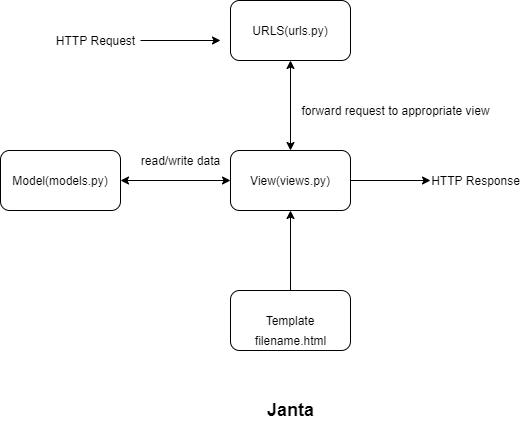
\includegraphics[width=14cm]{janta/jantaflow.png}
\end{figure}

\newpage

\section{Project Explanation}

\subsection{Homepage of Janta}
People can register or login.
\begin{figure}[htp]
    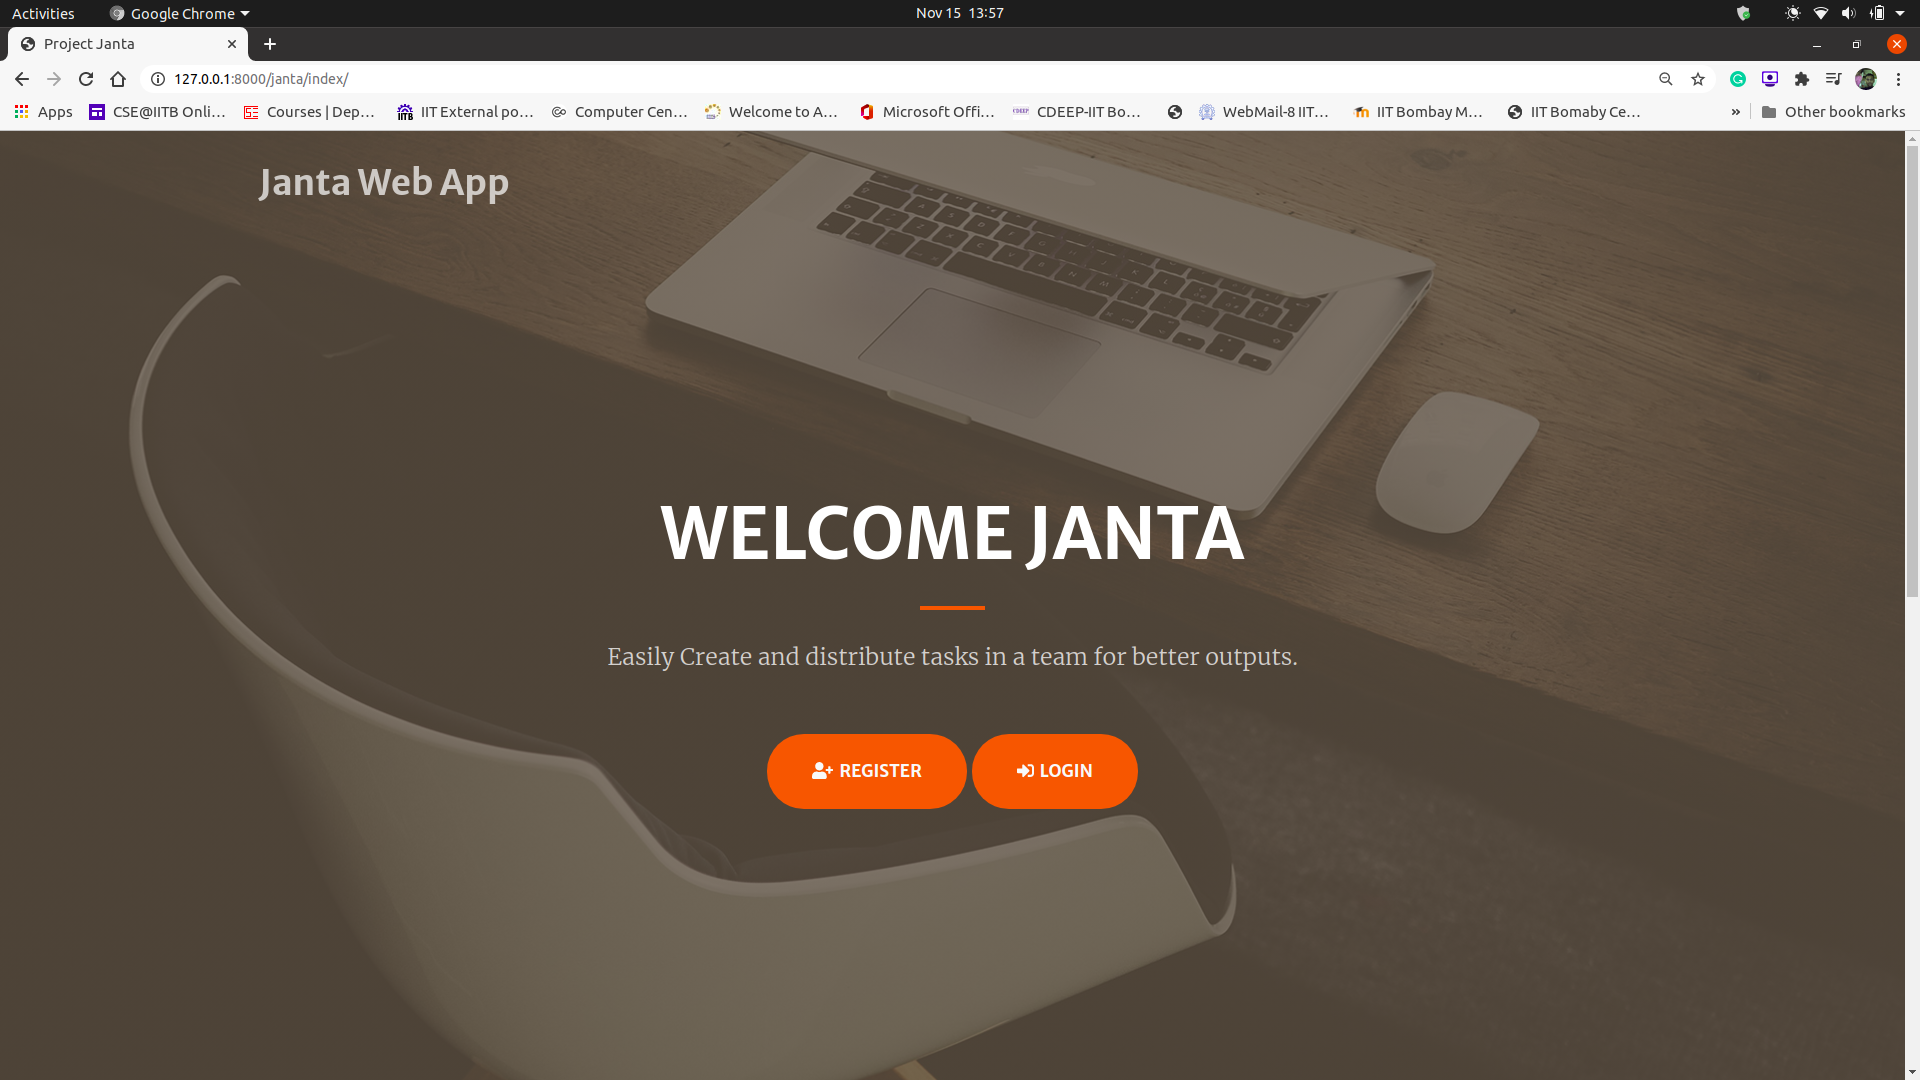
\includegraphics[width=12cm]{janta/Homepage.png}
\end{figure}
\\
\subsection{Register as user or moderator}
\begin{figure}[htp]
    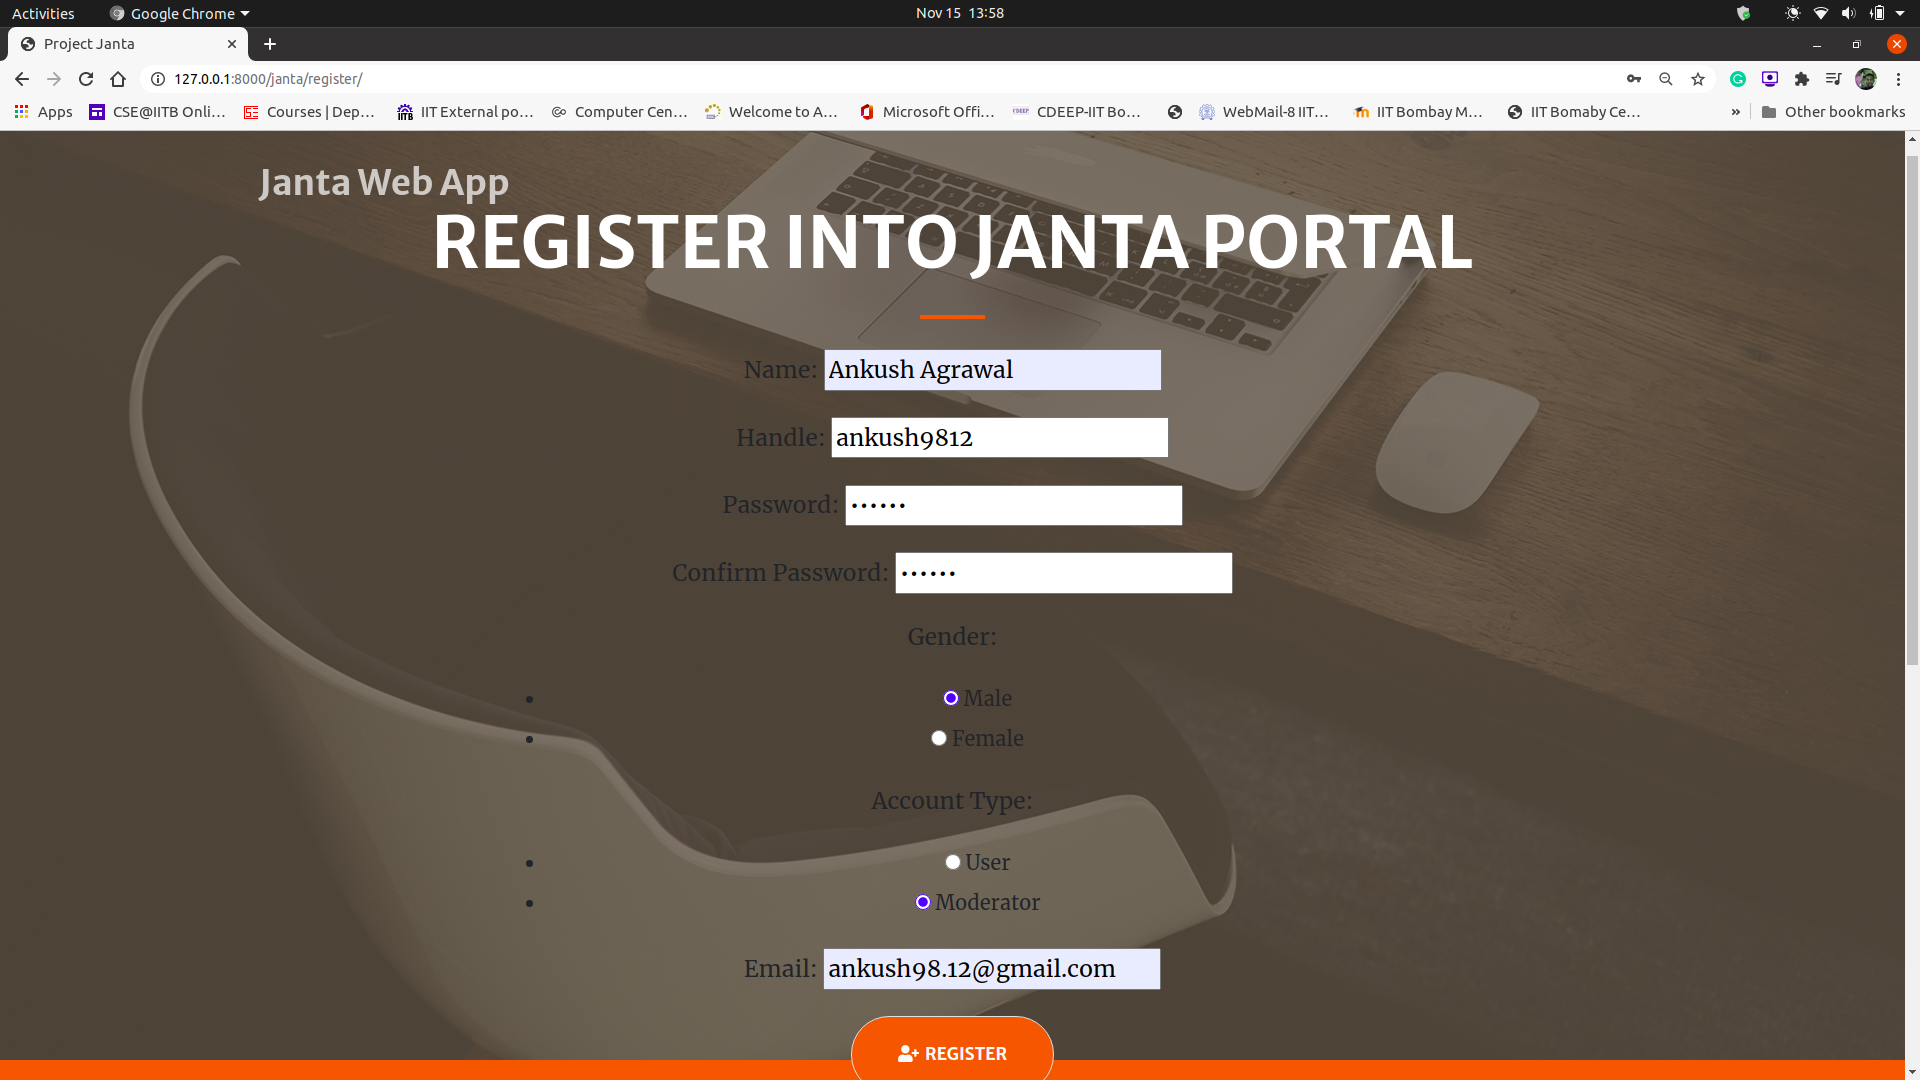
\includegraphics[width=12cm]{janta/Register.png}
\end{figure}
\newpage
\subsection{Login}
After registering,you will be redirected to login page.
\begin{figure}[htp]
    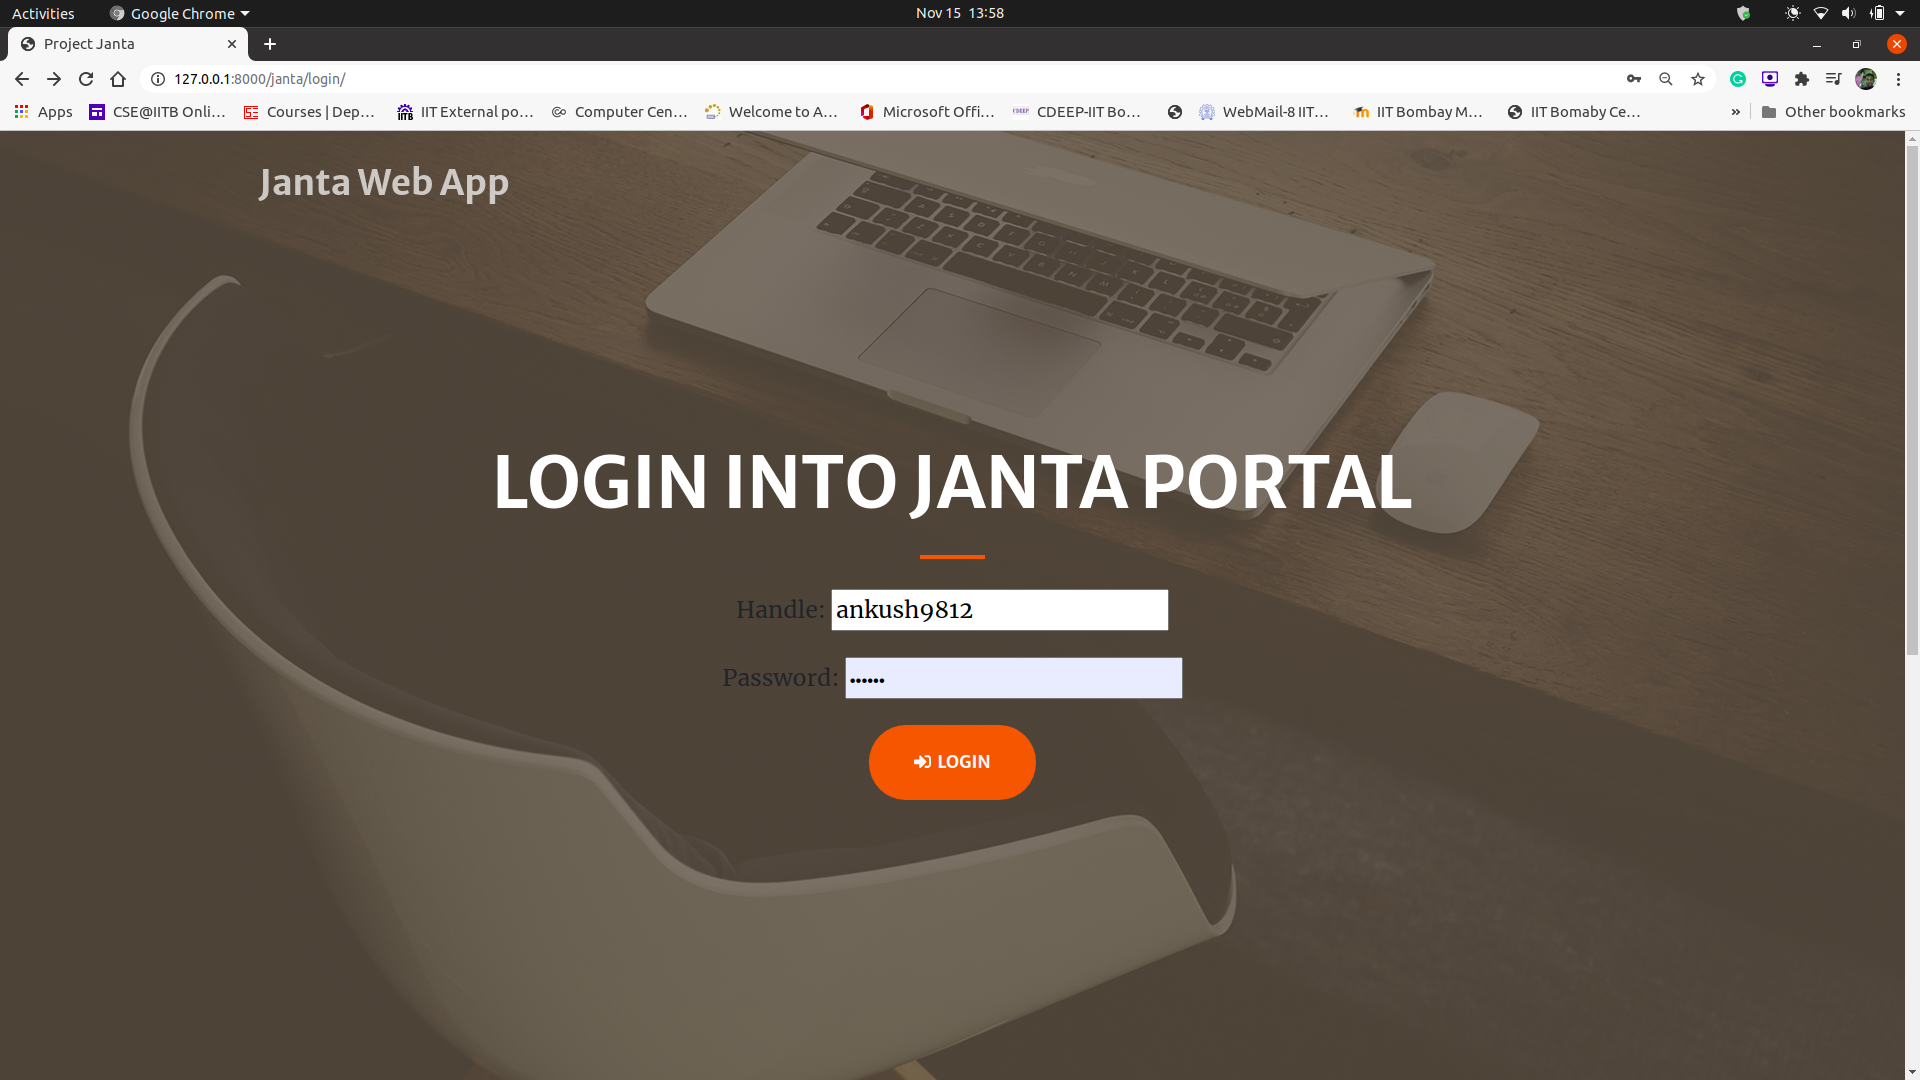
\includegraphics[width=15cm]{janta/Login.png}
\end{figure}
\newpage
\subsection{Moderator}
Moderator's Homepage.\\
Here moderator can assign task to user, delete the task and remove the assigned user from task.\\
Notification bar is present on every page.\\
\begin{figure}[htp]
    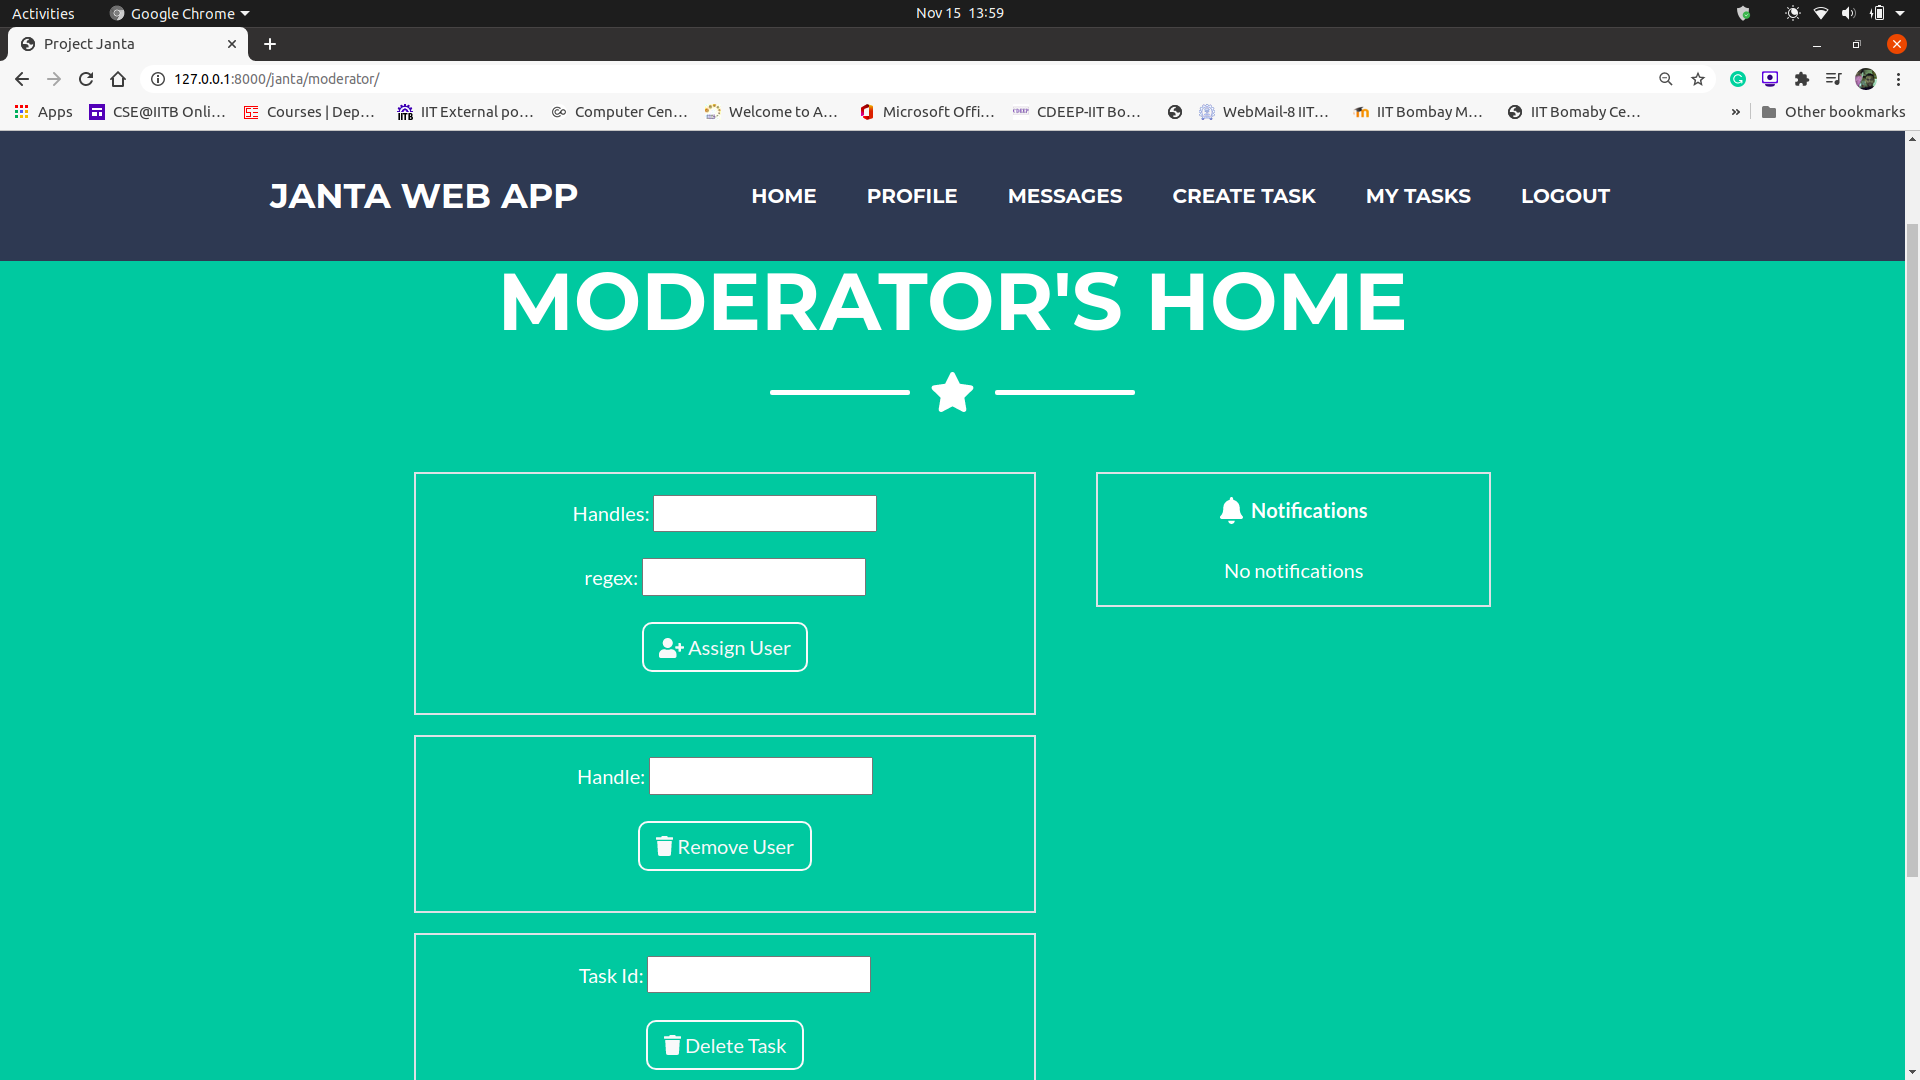
\includegraphics[width=15cm]{janta/Moderators_home.png}
\end{figure}
\newpage
It is the profile page of user or moderator. It gives the option to edit profile or change password.
\begin{figure}[htp]
    
\includegraphics[width=12cm]{janta/profile.png}
\end{figure}
\\
Moderator will create the task here. Task can be Info type, character input or file upload, we have provided the option to select.
\begin{figure}[htp]
    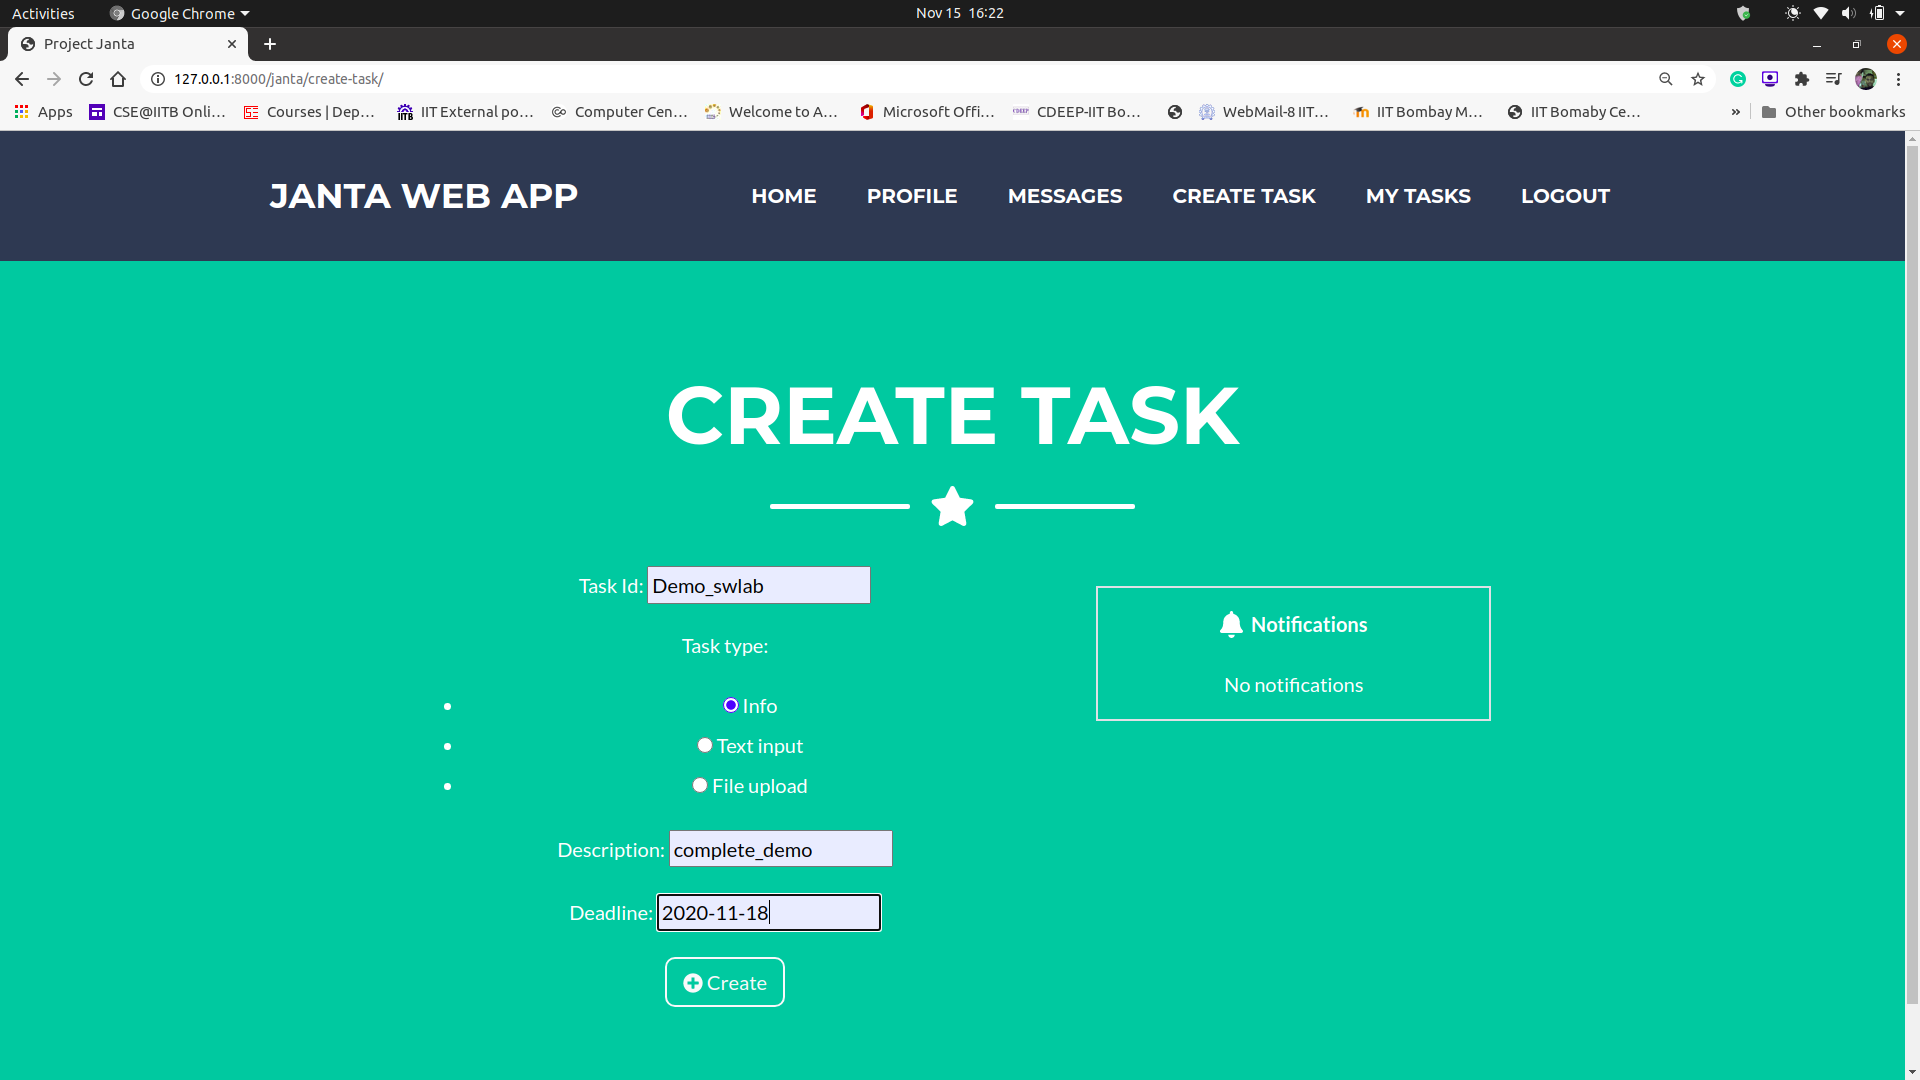
\includegraphics[width=12cm]{janta/create task.png}
\end{figure}

\newpage
It is the page to see the tasks created by moderator. Moderator can modify the task or check the task status.
\begin{figure}[htp]
    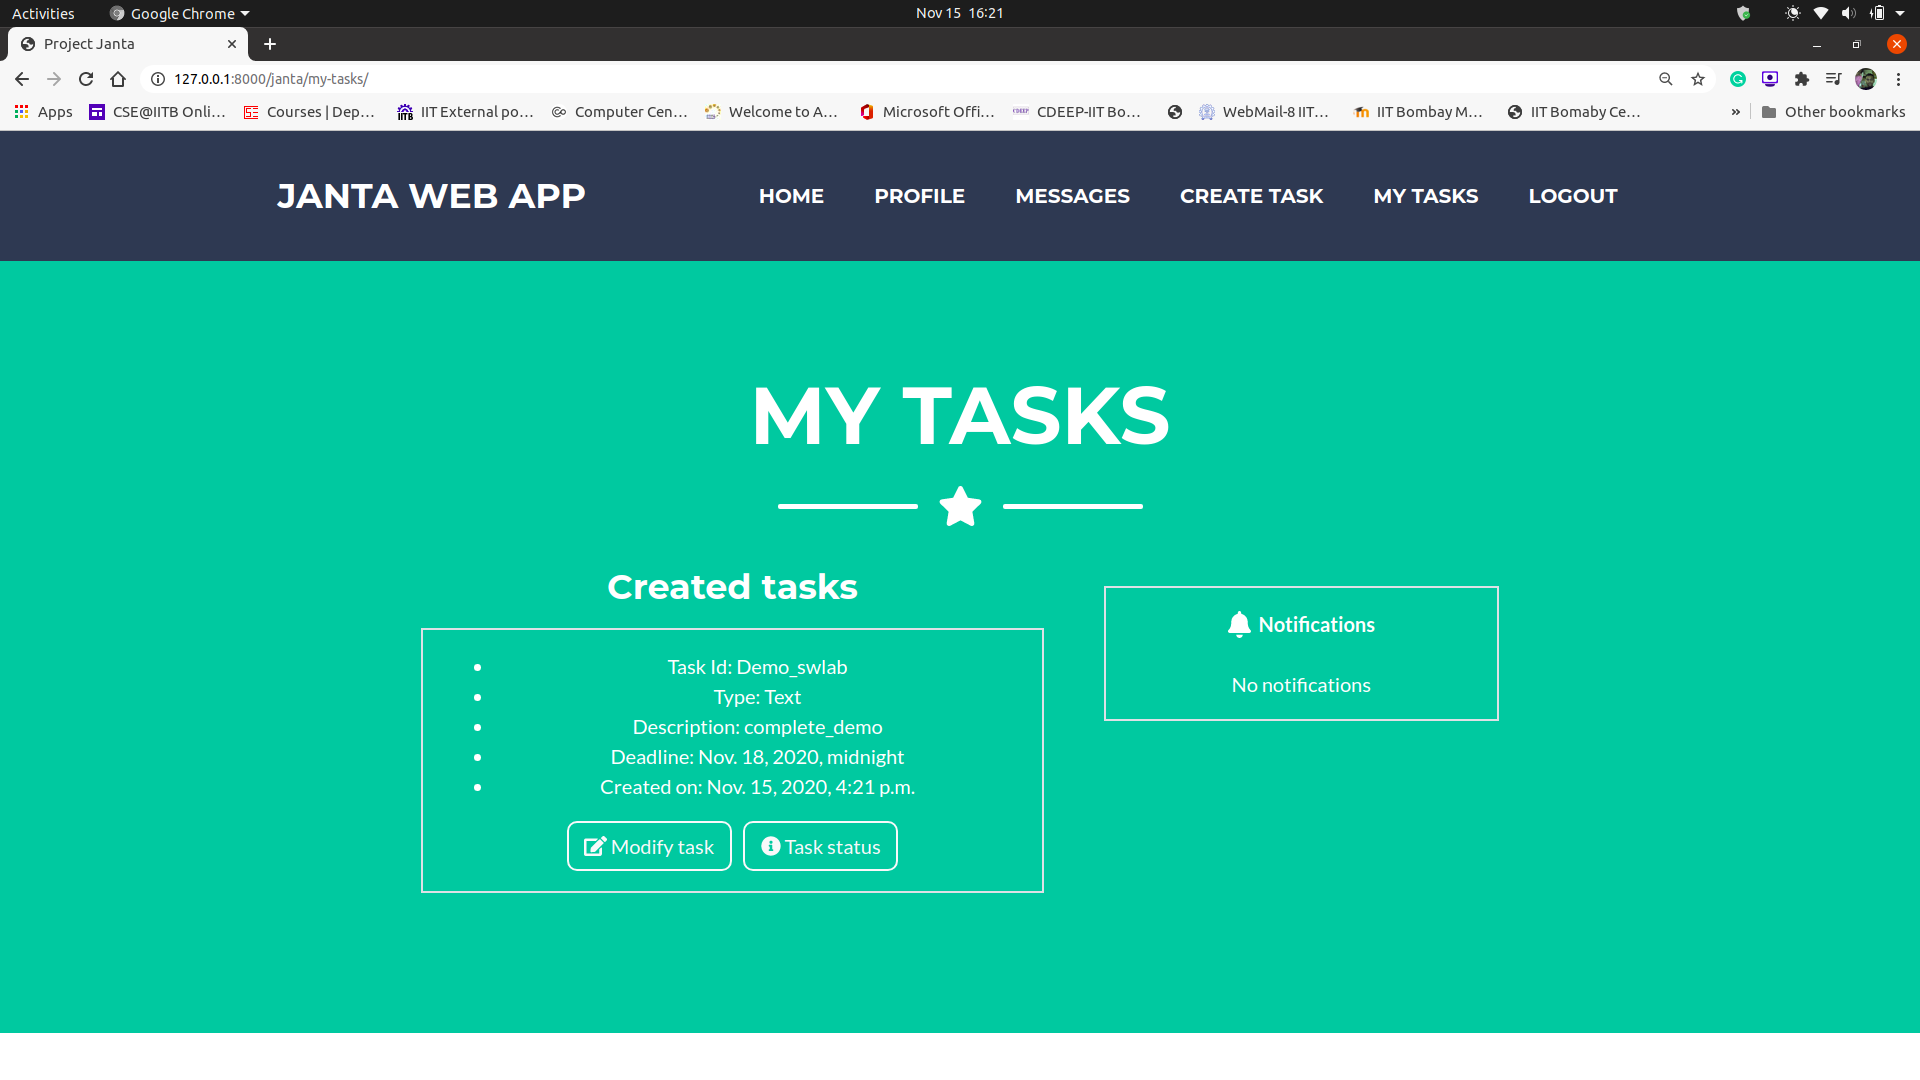
\includegraphics[width=12cm]{janta/mytasks.png}
\end{figure}
\\
Task status
\begin{figure}[htp]
    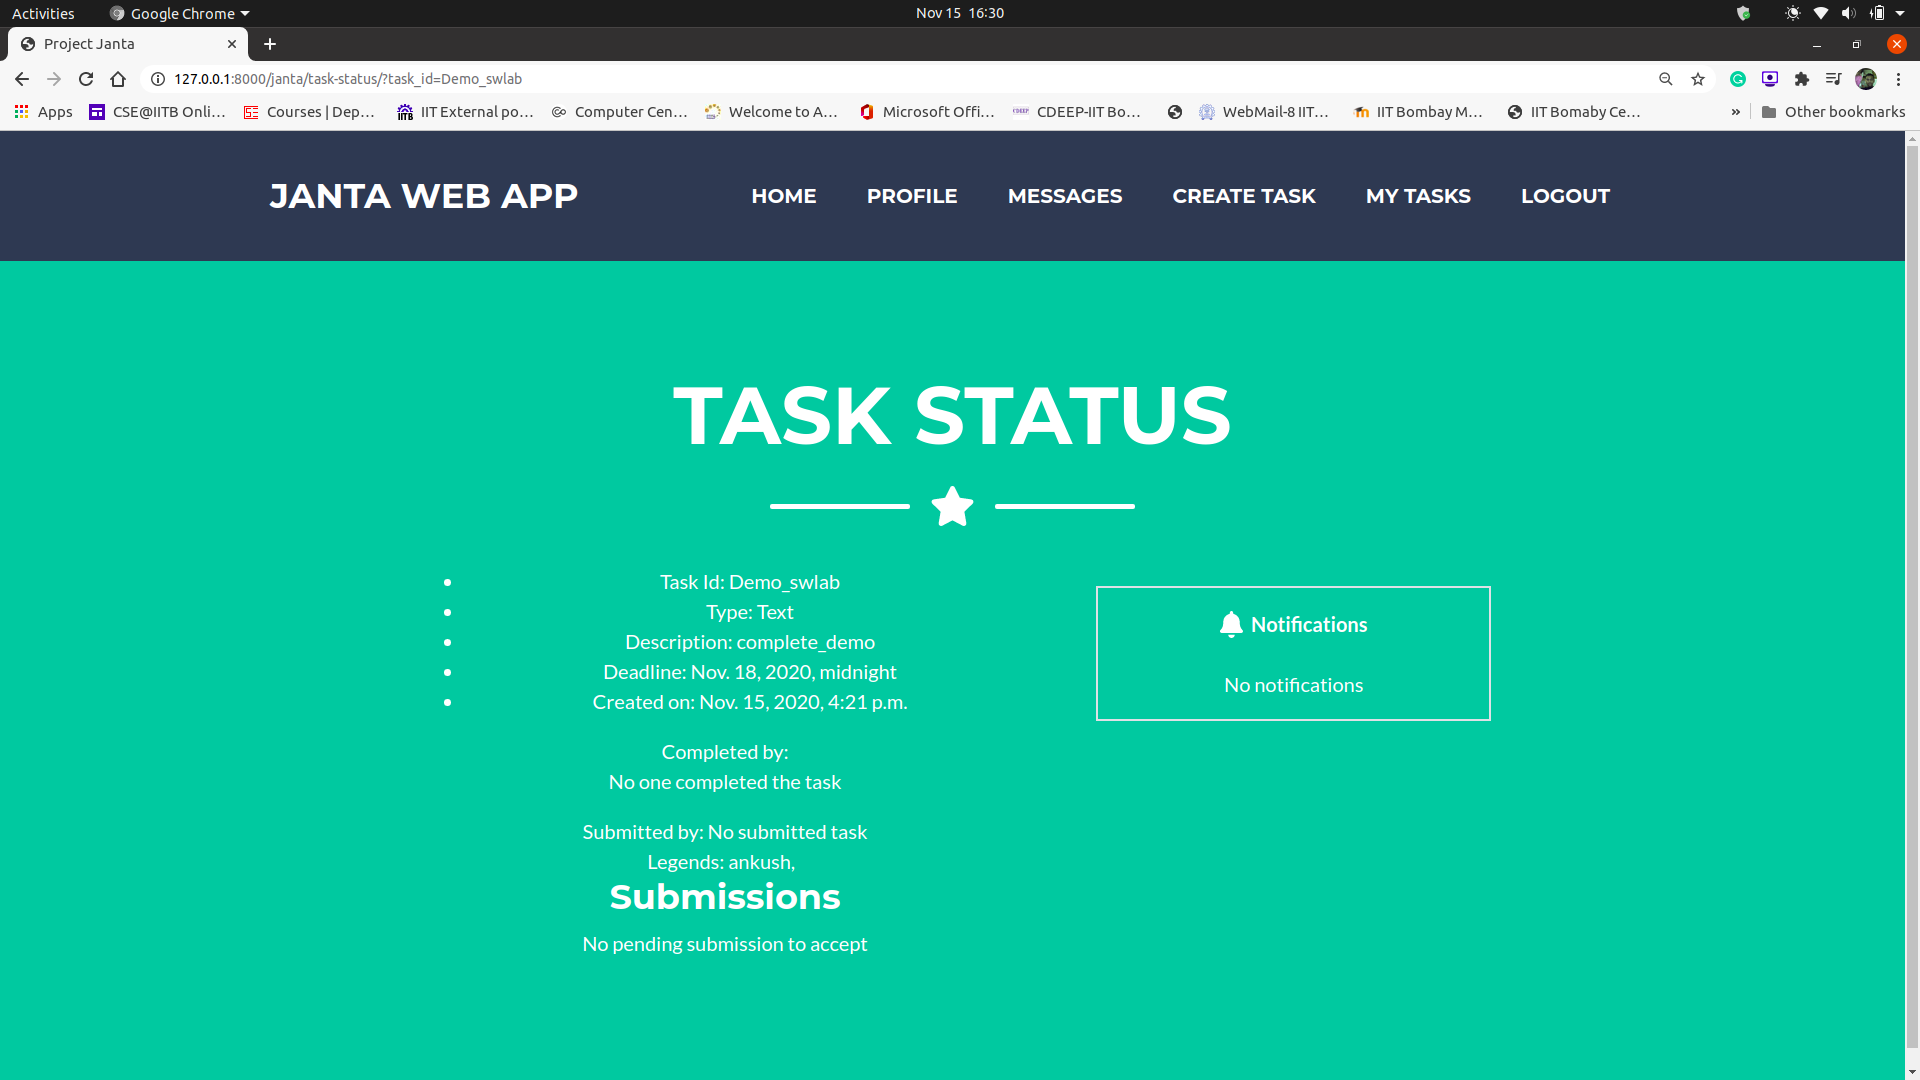
\includegraphics[width=12cm]{janta/task_status.png}
\end{figure}
\newpage
Messages can be sent to users.
\begin{figure}[htp]
    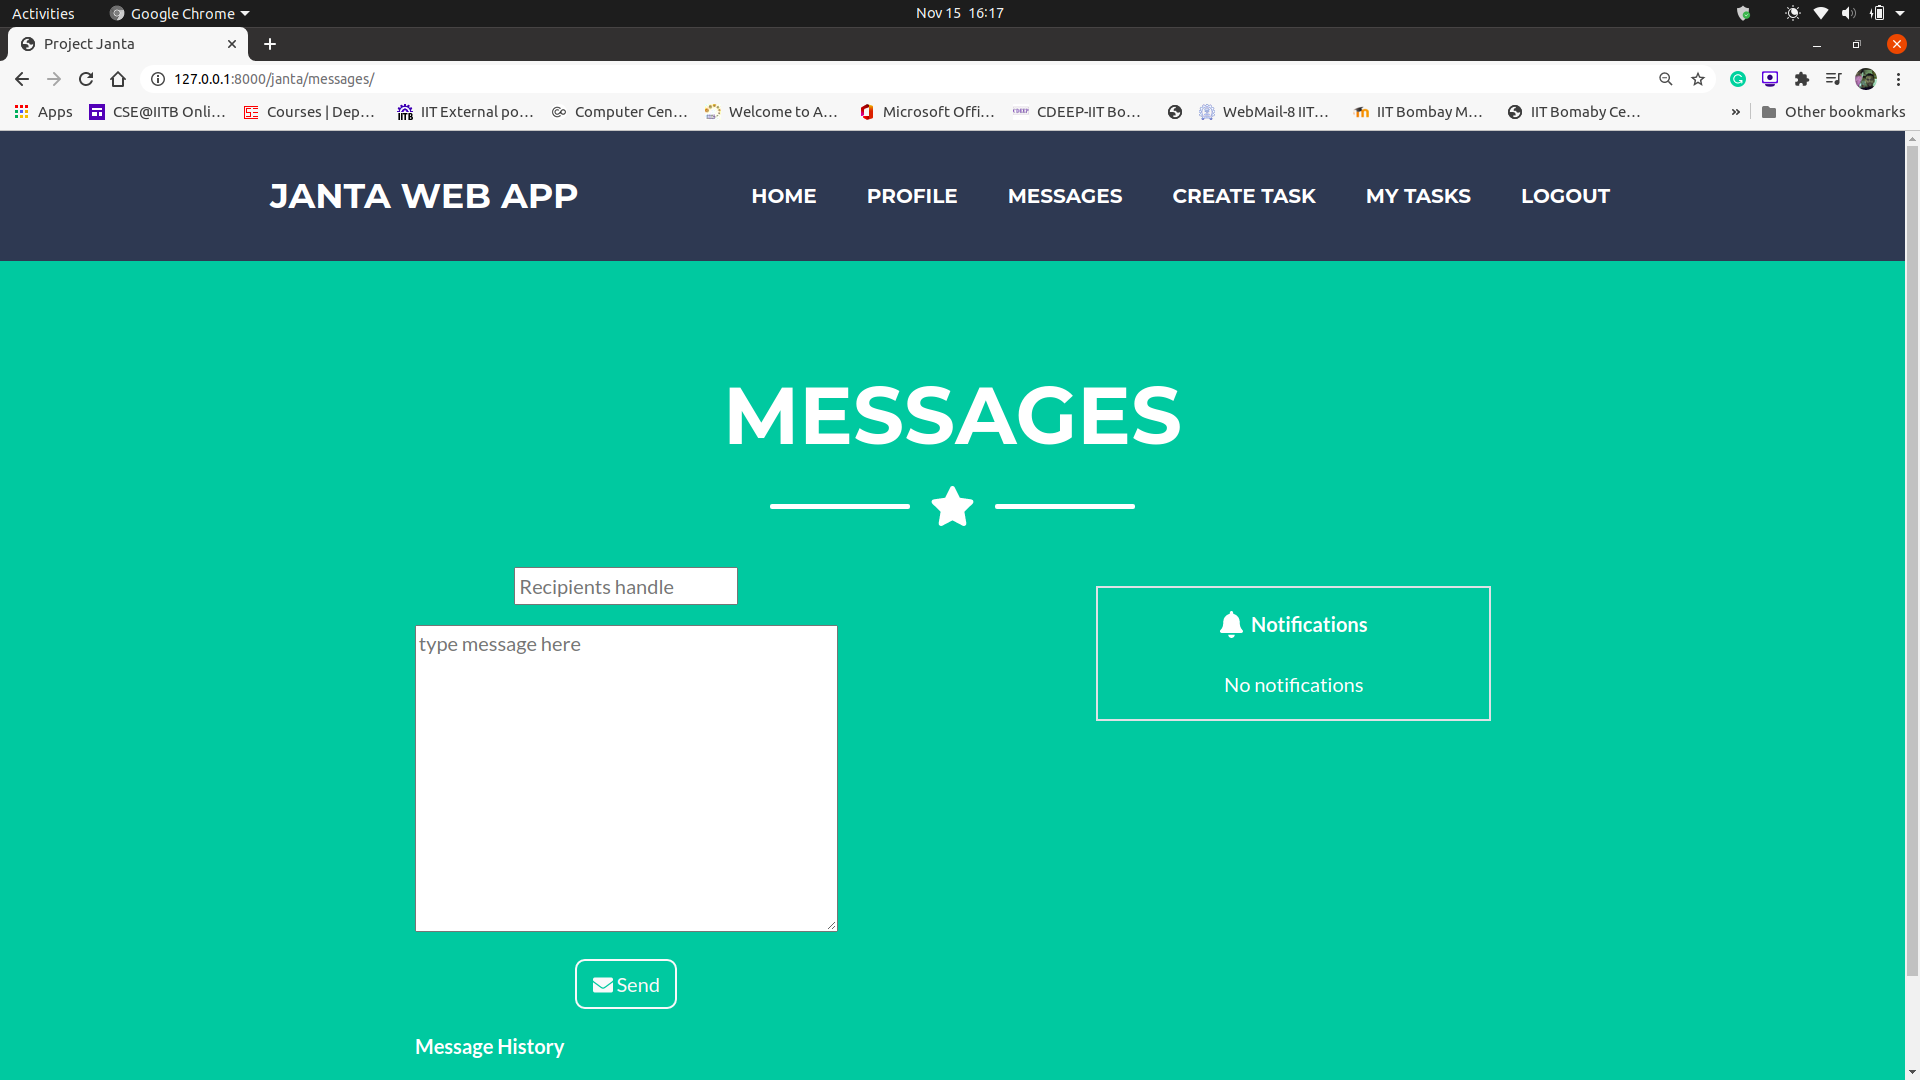
\includegraphics[width=12cm]{janta/messages.png}
\end{figure}
\\
The logout option is present.

\subsection{User}
User's homepage where recently assigned tasks and notifications will be shown.
\begin{figure}[htp]
    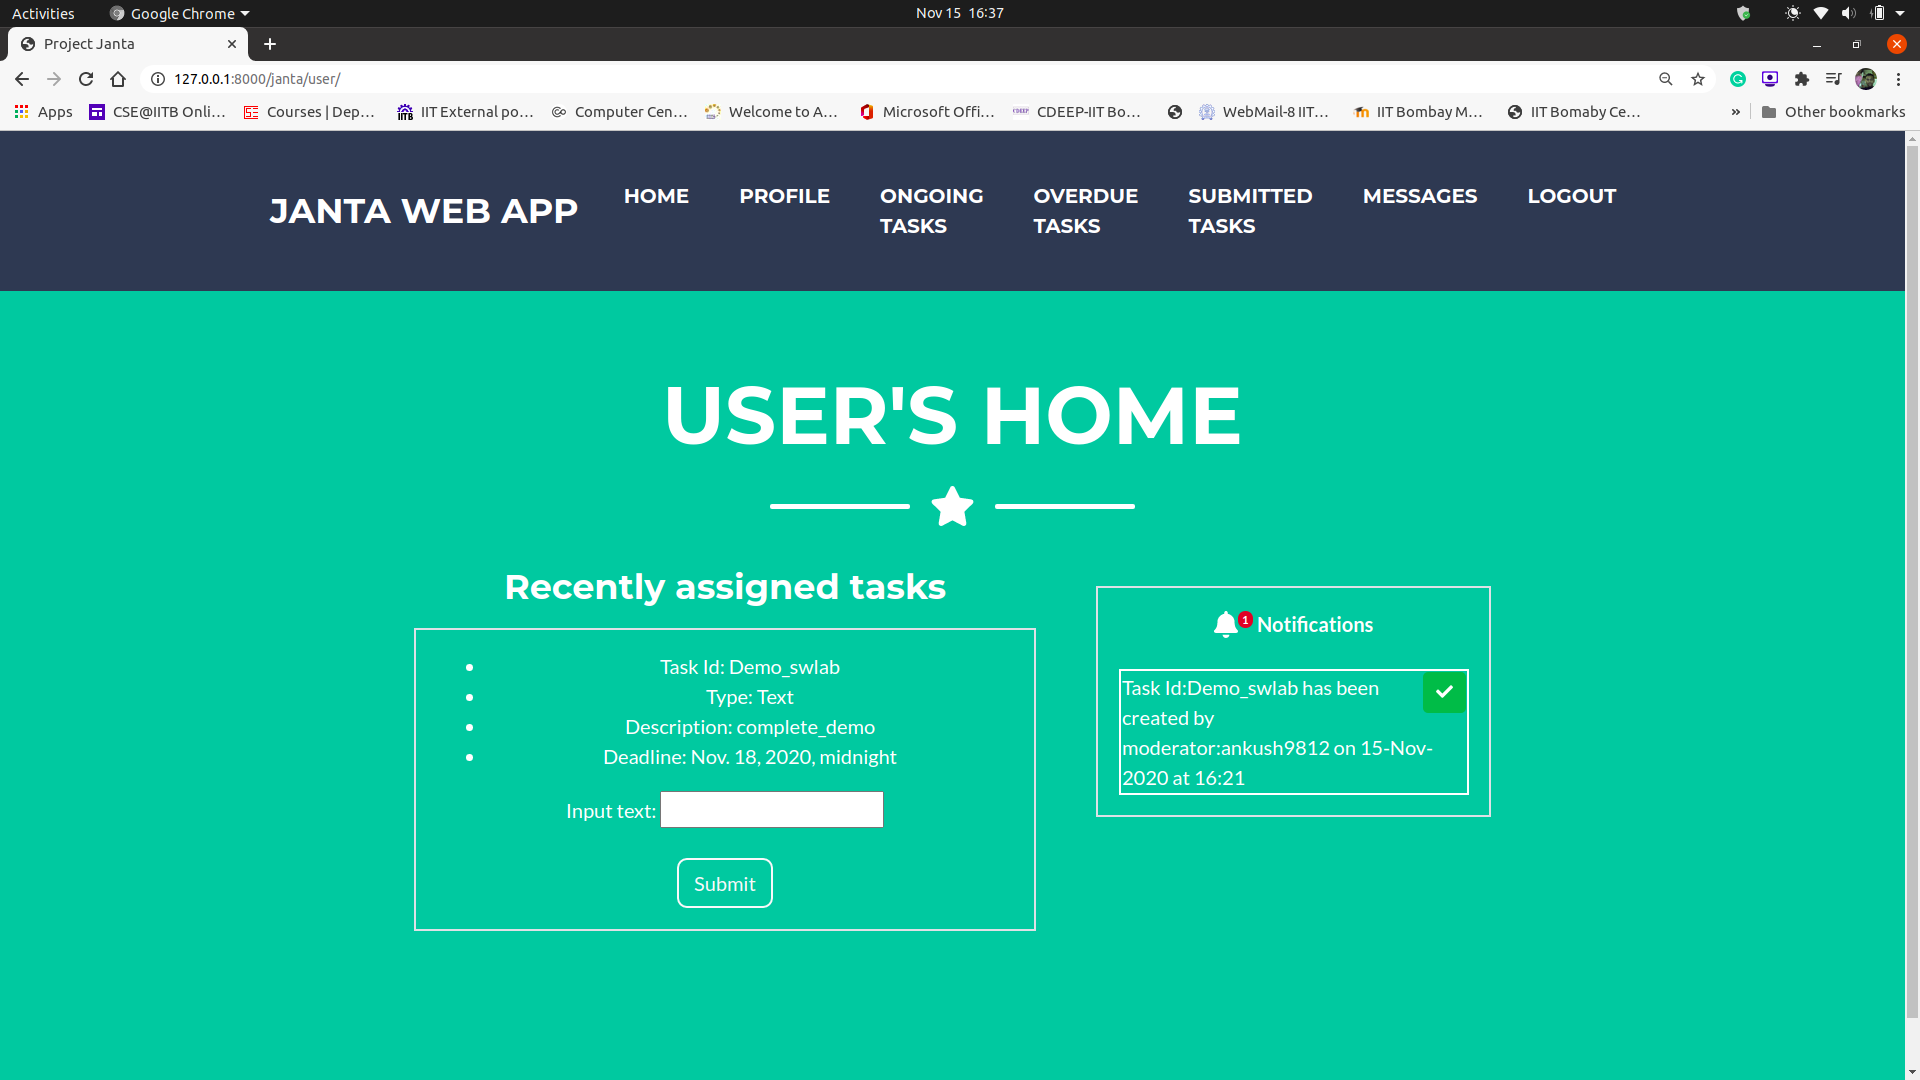
\includegraphics[width=12cm]{janta/users_home.png}
\end{figure}
\newpage
User's ongoing tasks, for which user has time to submit the task.
\begin{figure}[htp]
    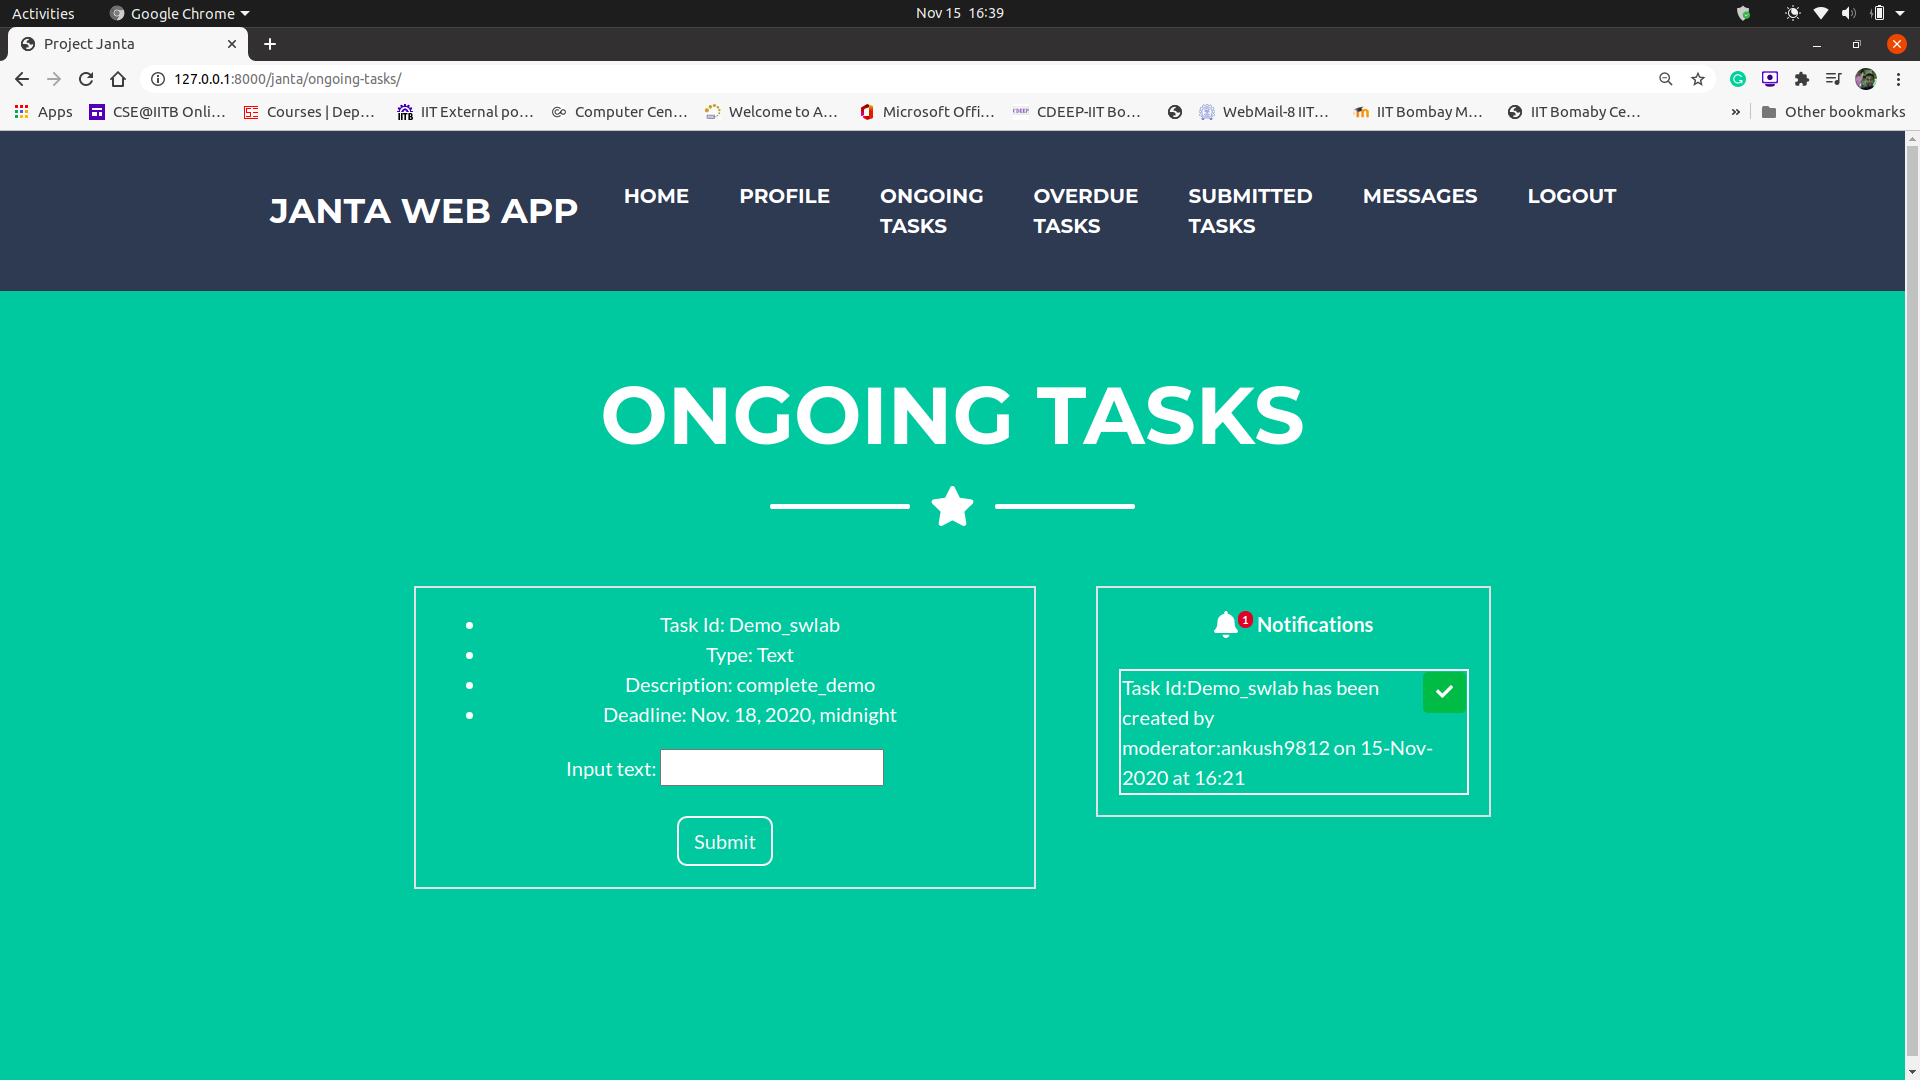
\includegraphics[width=12cm]{janta/ongoing_tasks.png}
\end{figure}
\\
User's overdue tasks whose deadline had passed will be shown.
\begin{figure}[htp]
    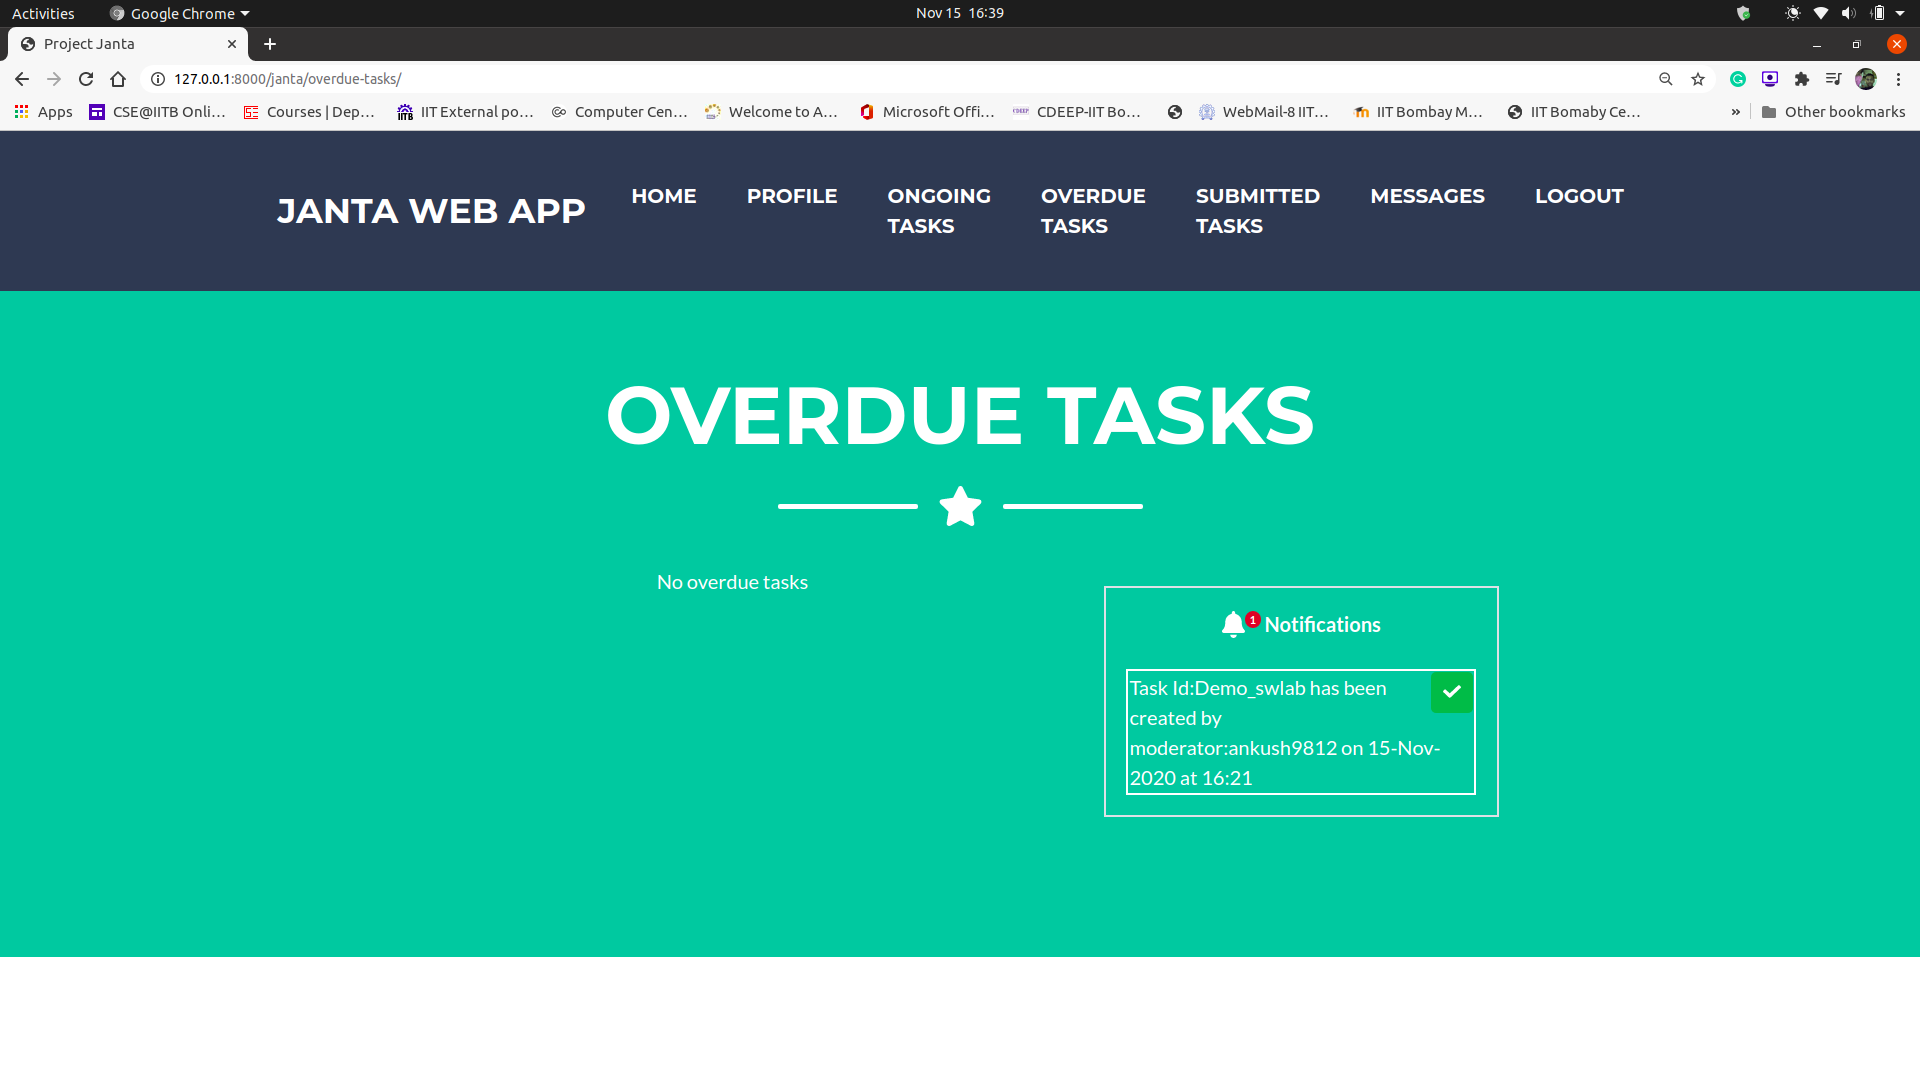
\includegraphics[width=12cm]{janta/overdue_tasks.png}
\end{figure}
\newpage
Submitted tasks of the user will be shown.
\begin{figure}[htp]
    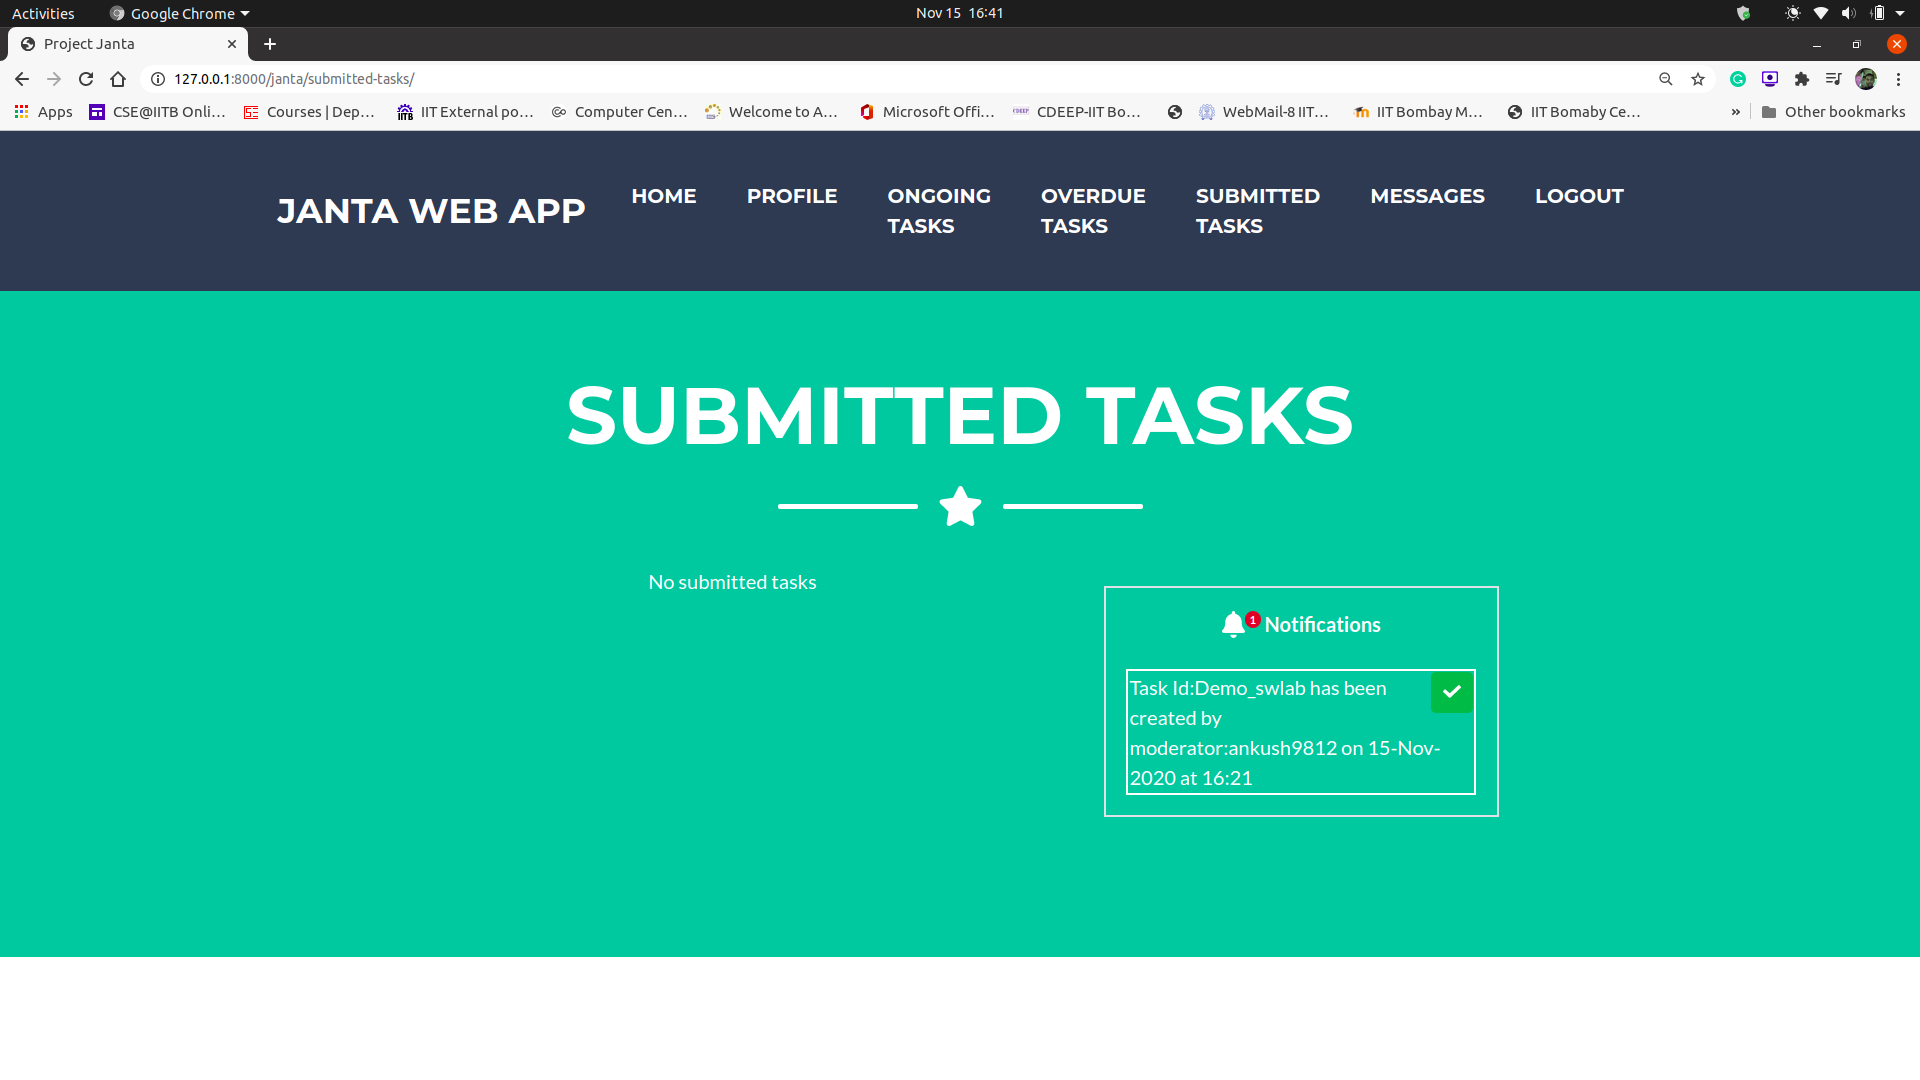
\includegraphics[width=12cm]{janta/submitted_tasks.png}
\end{figure}

\subsection{Admin}
This is the login page of admin. Admin has special functionalities.
\begin{figure}[htp]
    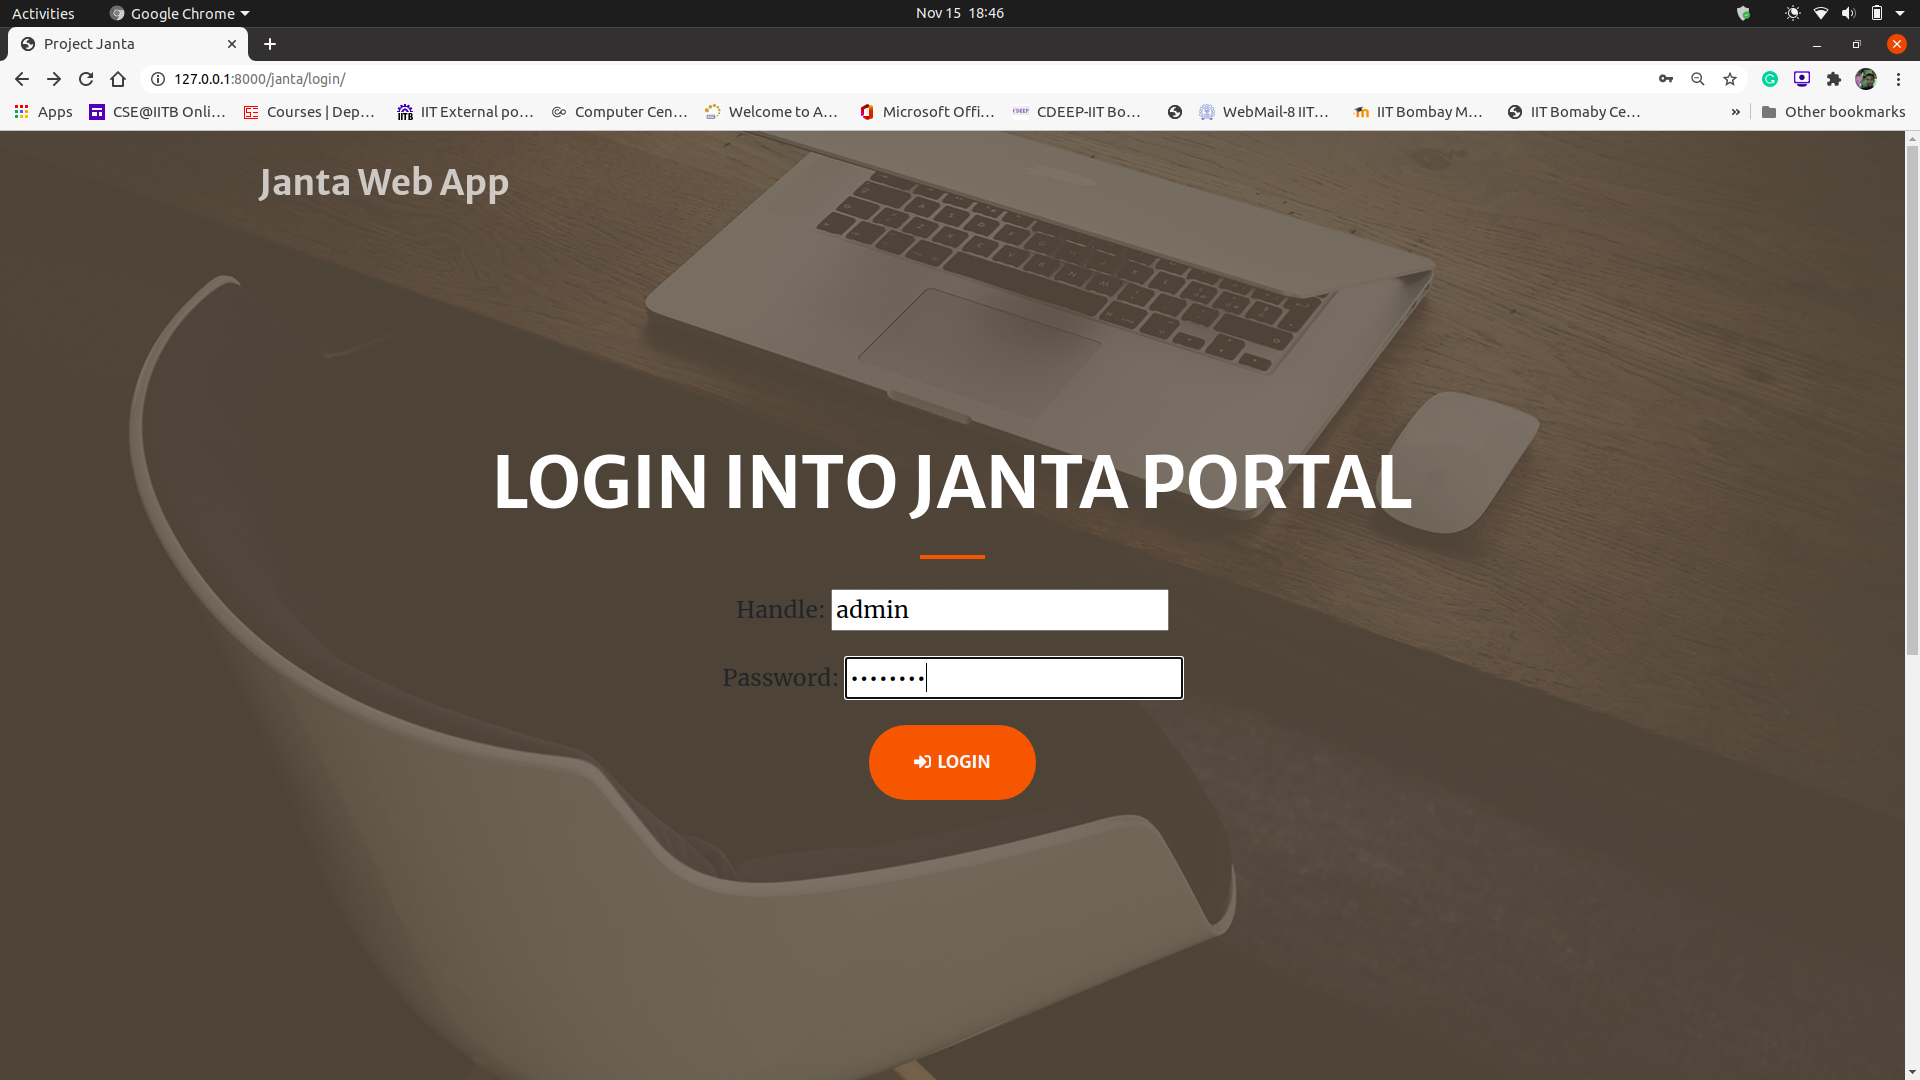
\includegraphics[width=12cm]{janta/admin.png}
\end{figure}
\newpage
This is the home page of admin where it can manage user, moderator or any task.\\
In the notifications it can be seen that attempt failed is notified. It is use to monitor any malicious user and strengthen our handle or password.
\begin{figure}[htp]
    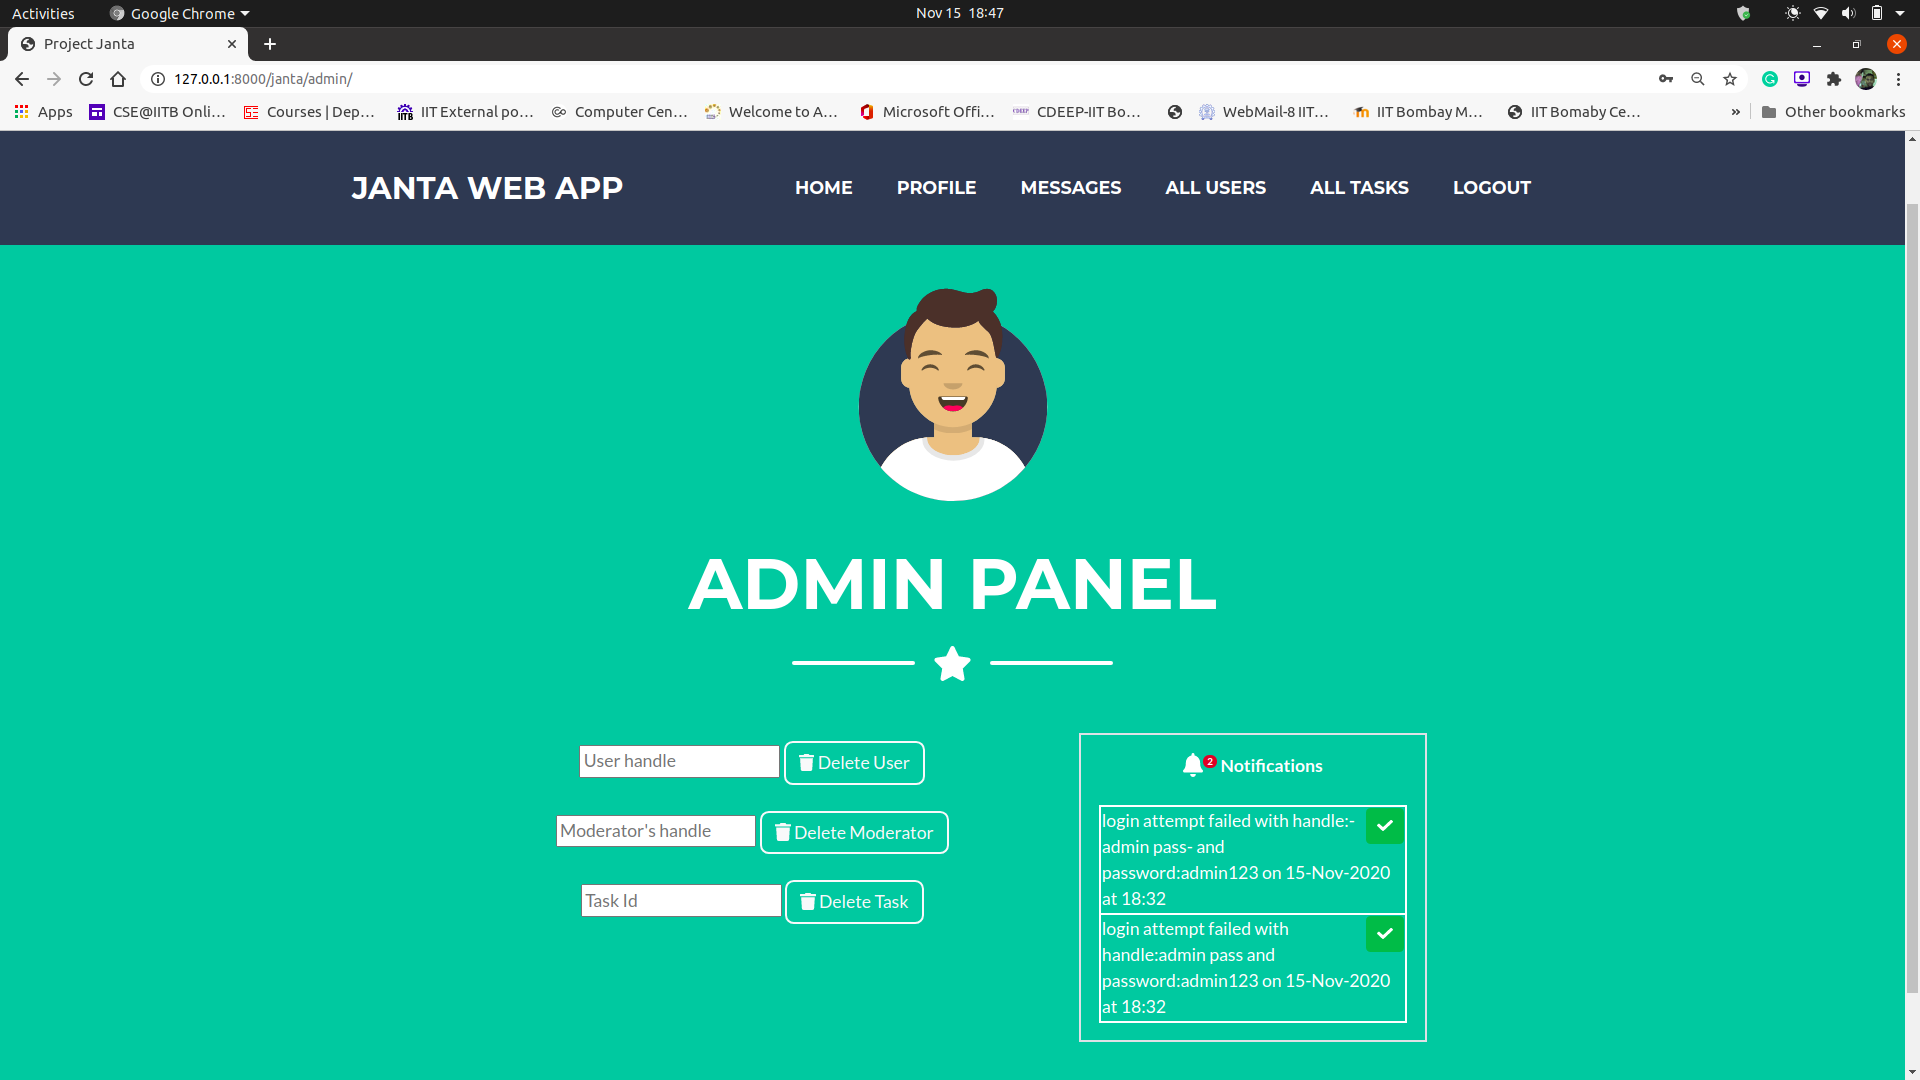
\includegraphics[width=12cm]{janta/admin_home.png}
\end{figure}
\\
This is ALL USERS page where all the registered users,moderators are shown and maintained.
\begin{figure}[htp]
    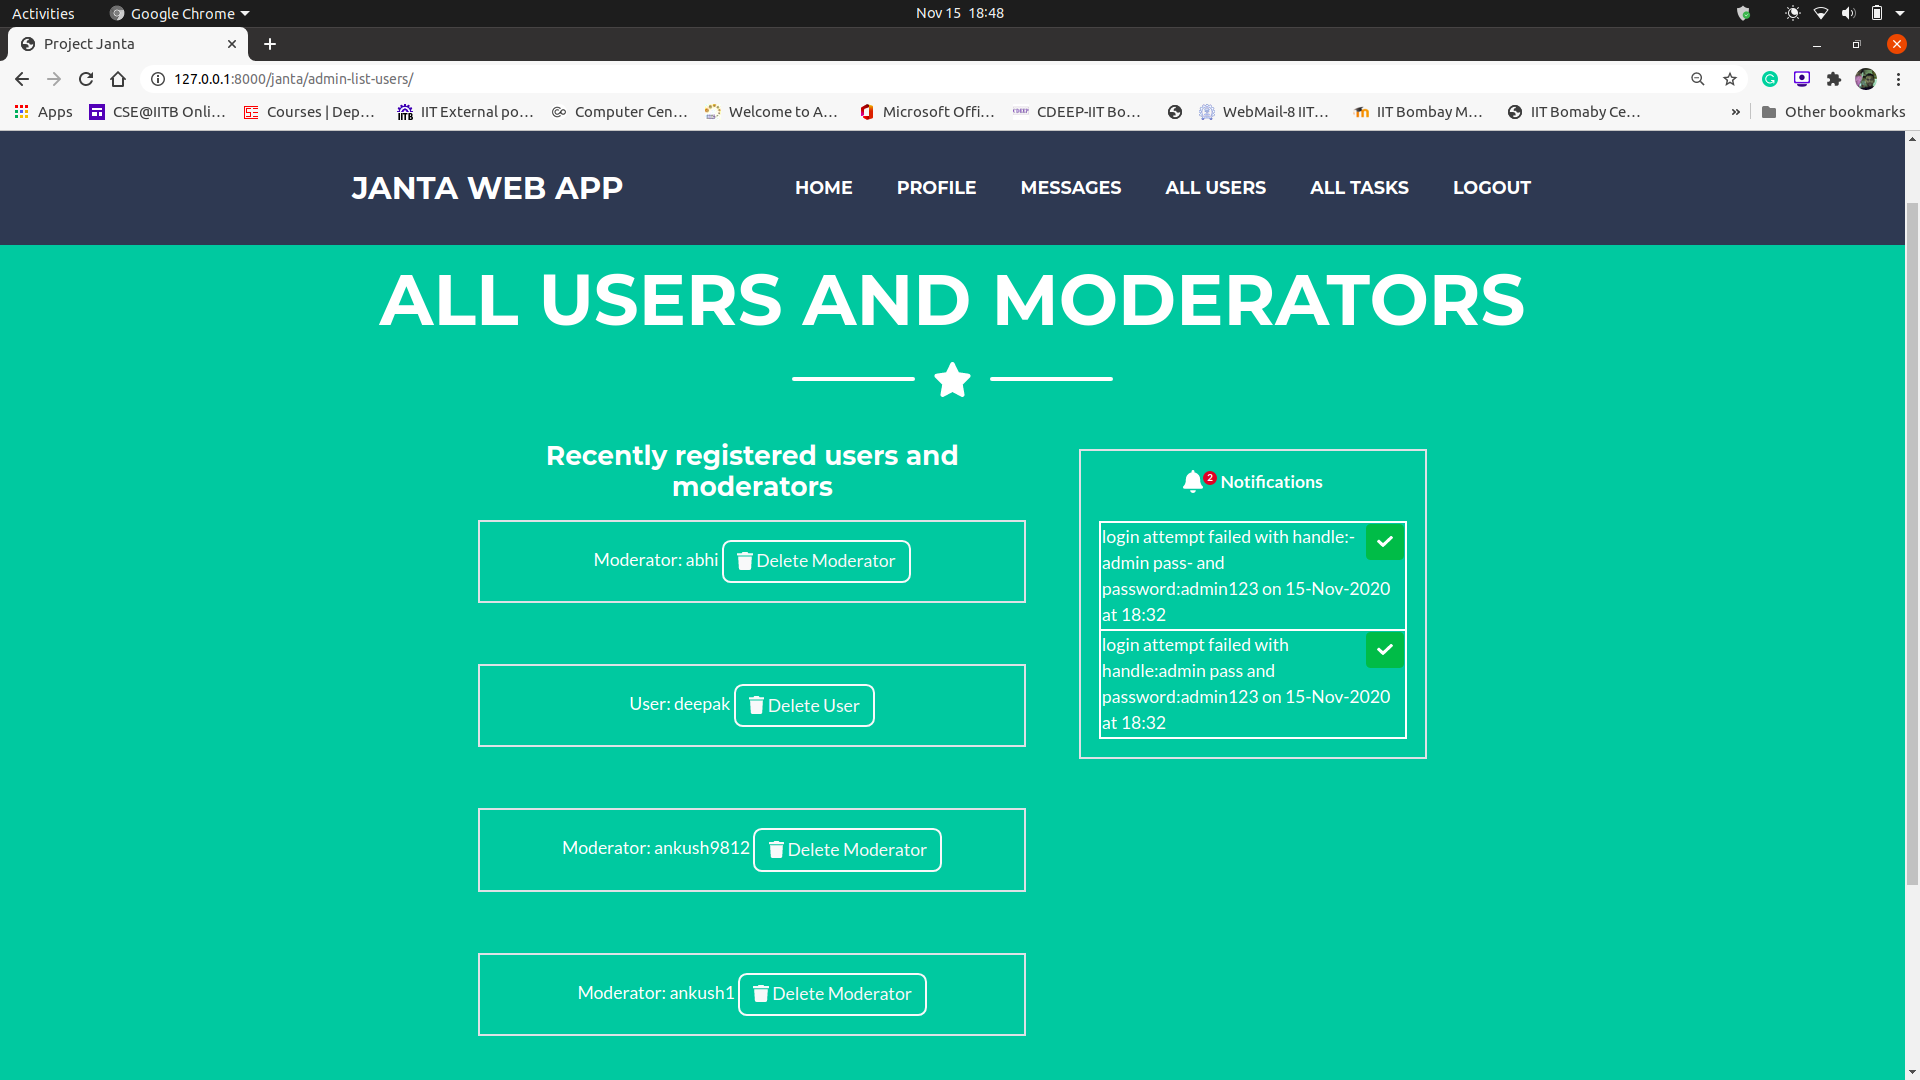
\includegraphics[width=12cm]{janta/admin_allusers.png}
\end{figure}
\newpage
This page shows all the created tasks.
\begin{figure}[htp]
    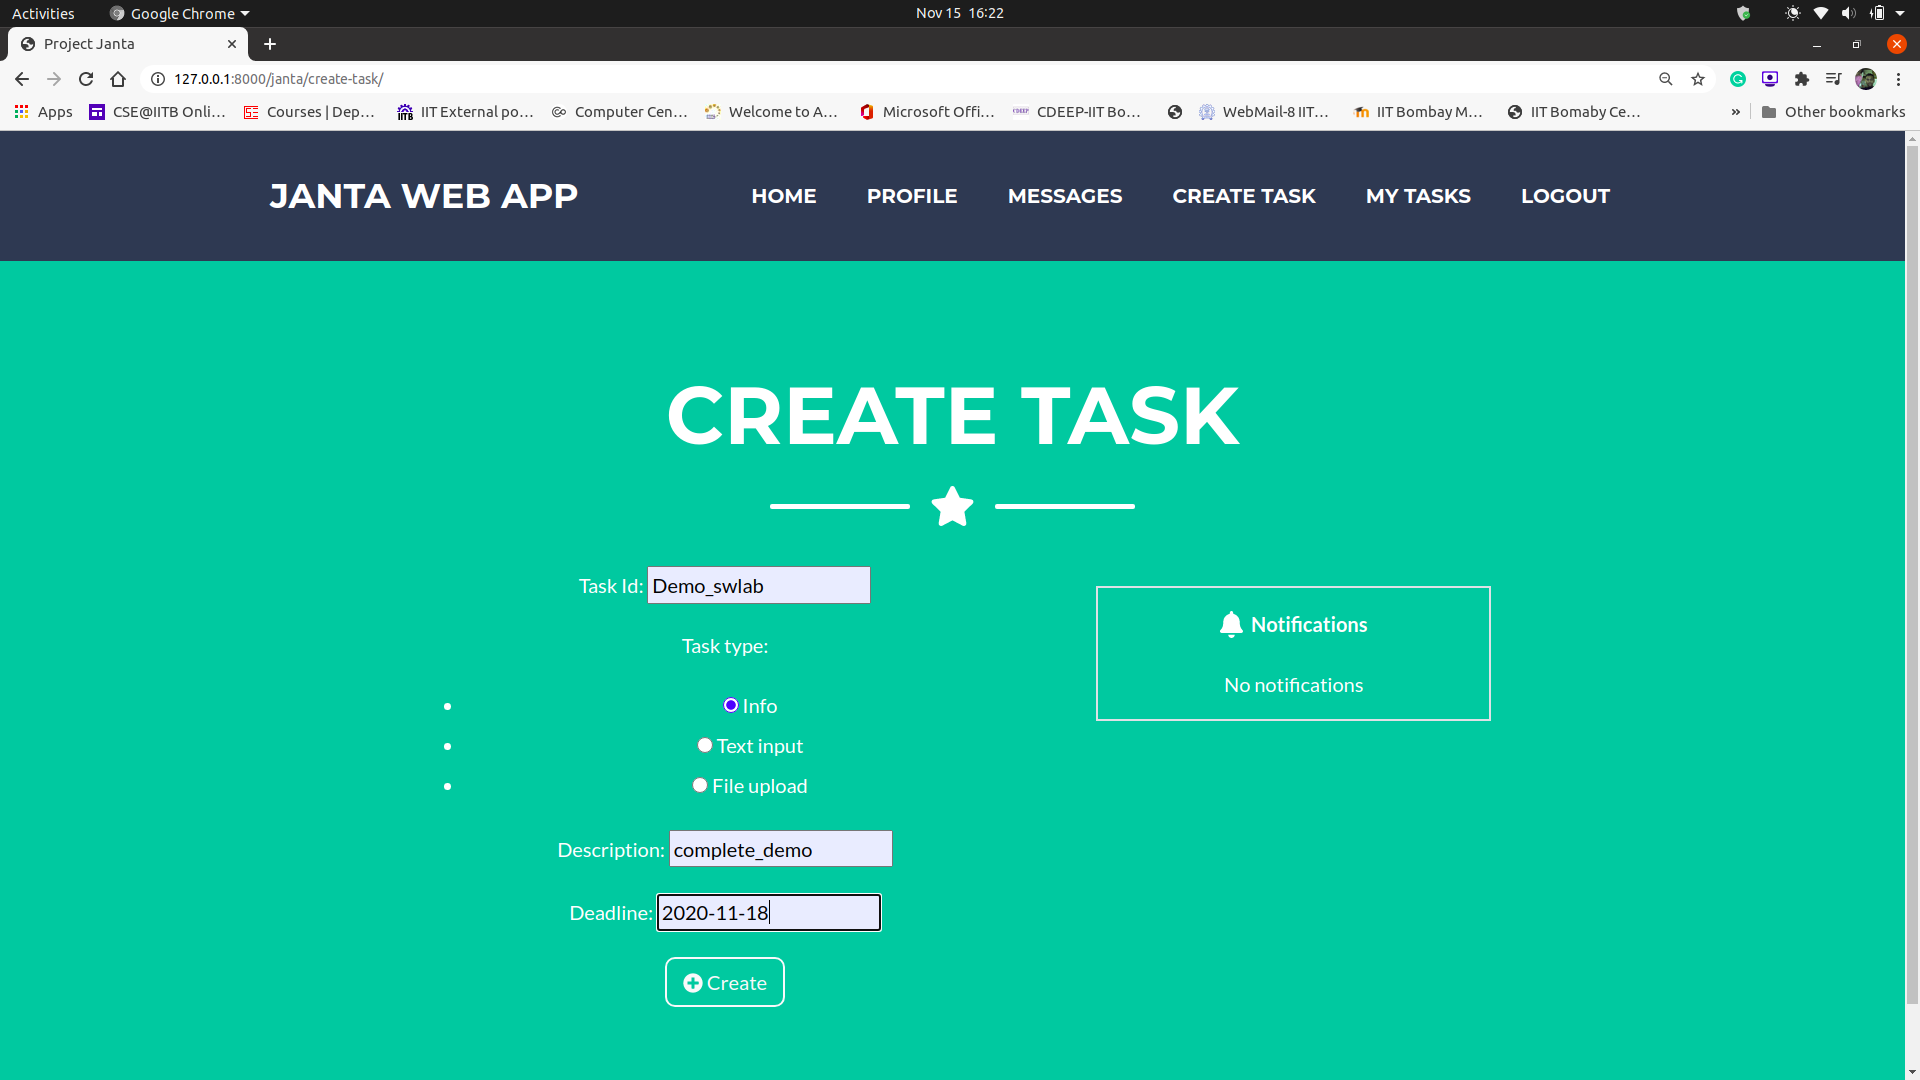
\includegraphics[width=12cm]{janta/create task.png}
\end{figure}
\newpage

\section{Future Scope}
\Large{Since the beginning of pandemic, people are scattered at different places so collaboration among team-members has dropped. This web application is useful for people who want to collaborate in a team and work on a job from different places.\\
Most of the work done among people of different age groups or employees of almost every company requires team-work and hence this app can be extended and used in all areas.\\
We have developed the application \textbf{JANTA} which is easy to use and easy to understand for team collaboration.}
\end{document}

